% \section{Актуальность темы}
\begin{frame}
    {Актуальность темы}
    \justifying

    Создание современной инфраструктуры передачи данных вдоль транспортных магистралей является одной из важнейших проблем при создании нового и функционировании существующего транспортного комплекса. 


    \bigskip

    Одним из путей решения проблемы является интенсивное развитие и внедрение беспроводных технологий.
    \bigskip


    Активное использование беспроводных сетей основывается на ряде их преимуществ по сравнению с кабельными сетями:
    \begin{itemize}
        \item возможность организации связи в труднодоступных регионах;
        \item быстрый ввод в эксплуатацию;
        \item сокращение капитальных затрат на создание и эксплуатацию сети; 
        \item высокая гибкость, мобильность, масштабируемость.
    \end{itemize}

    
\end{frame}

% \begin{frame}
%     {Актуальность темы}
%     \justifying
%     Активное использование беспроводных сетей основывается на ряде их преимуществ по сравнению с кабельными сетями:
%     \begin{itemize}
%         \item возможность получения информации с любой точки контролируемой территории;
%         \item быстрый ввод в эксплуатацию по системе подключение типа Plug-\&-Play;
%         \item сокращение капитальных затрат на создание сети; 
%         \item уменьшение затрат на эксплуатацию;
%         \item высокая гибкость, мобильность, масштабируемость;
%         \item упрощенные требования к обслуживанию оборудования.
%     \end{itemize}

% \end{frame}

% \section{Научно-техническая проблема}
\begin{frame}
    {Научно-техническая проблема}
    \justifying

    В рамках этого процесса возникает актуальная научно - техническая проблема \textbf{повышения качества проектирования беспроводной сети связи}, осуществляющей мониторинг, сбор и передачу информации в центр управления с множества объектов на заданной территории.  
 

\end{frame}


\begin{frame}
    {Научно-техническая проблема}
    Процесс проектирования БШС в общем виде состоит из последовательного решения взаимосвязанных задач:
    
    \bigskip

        
        \center{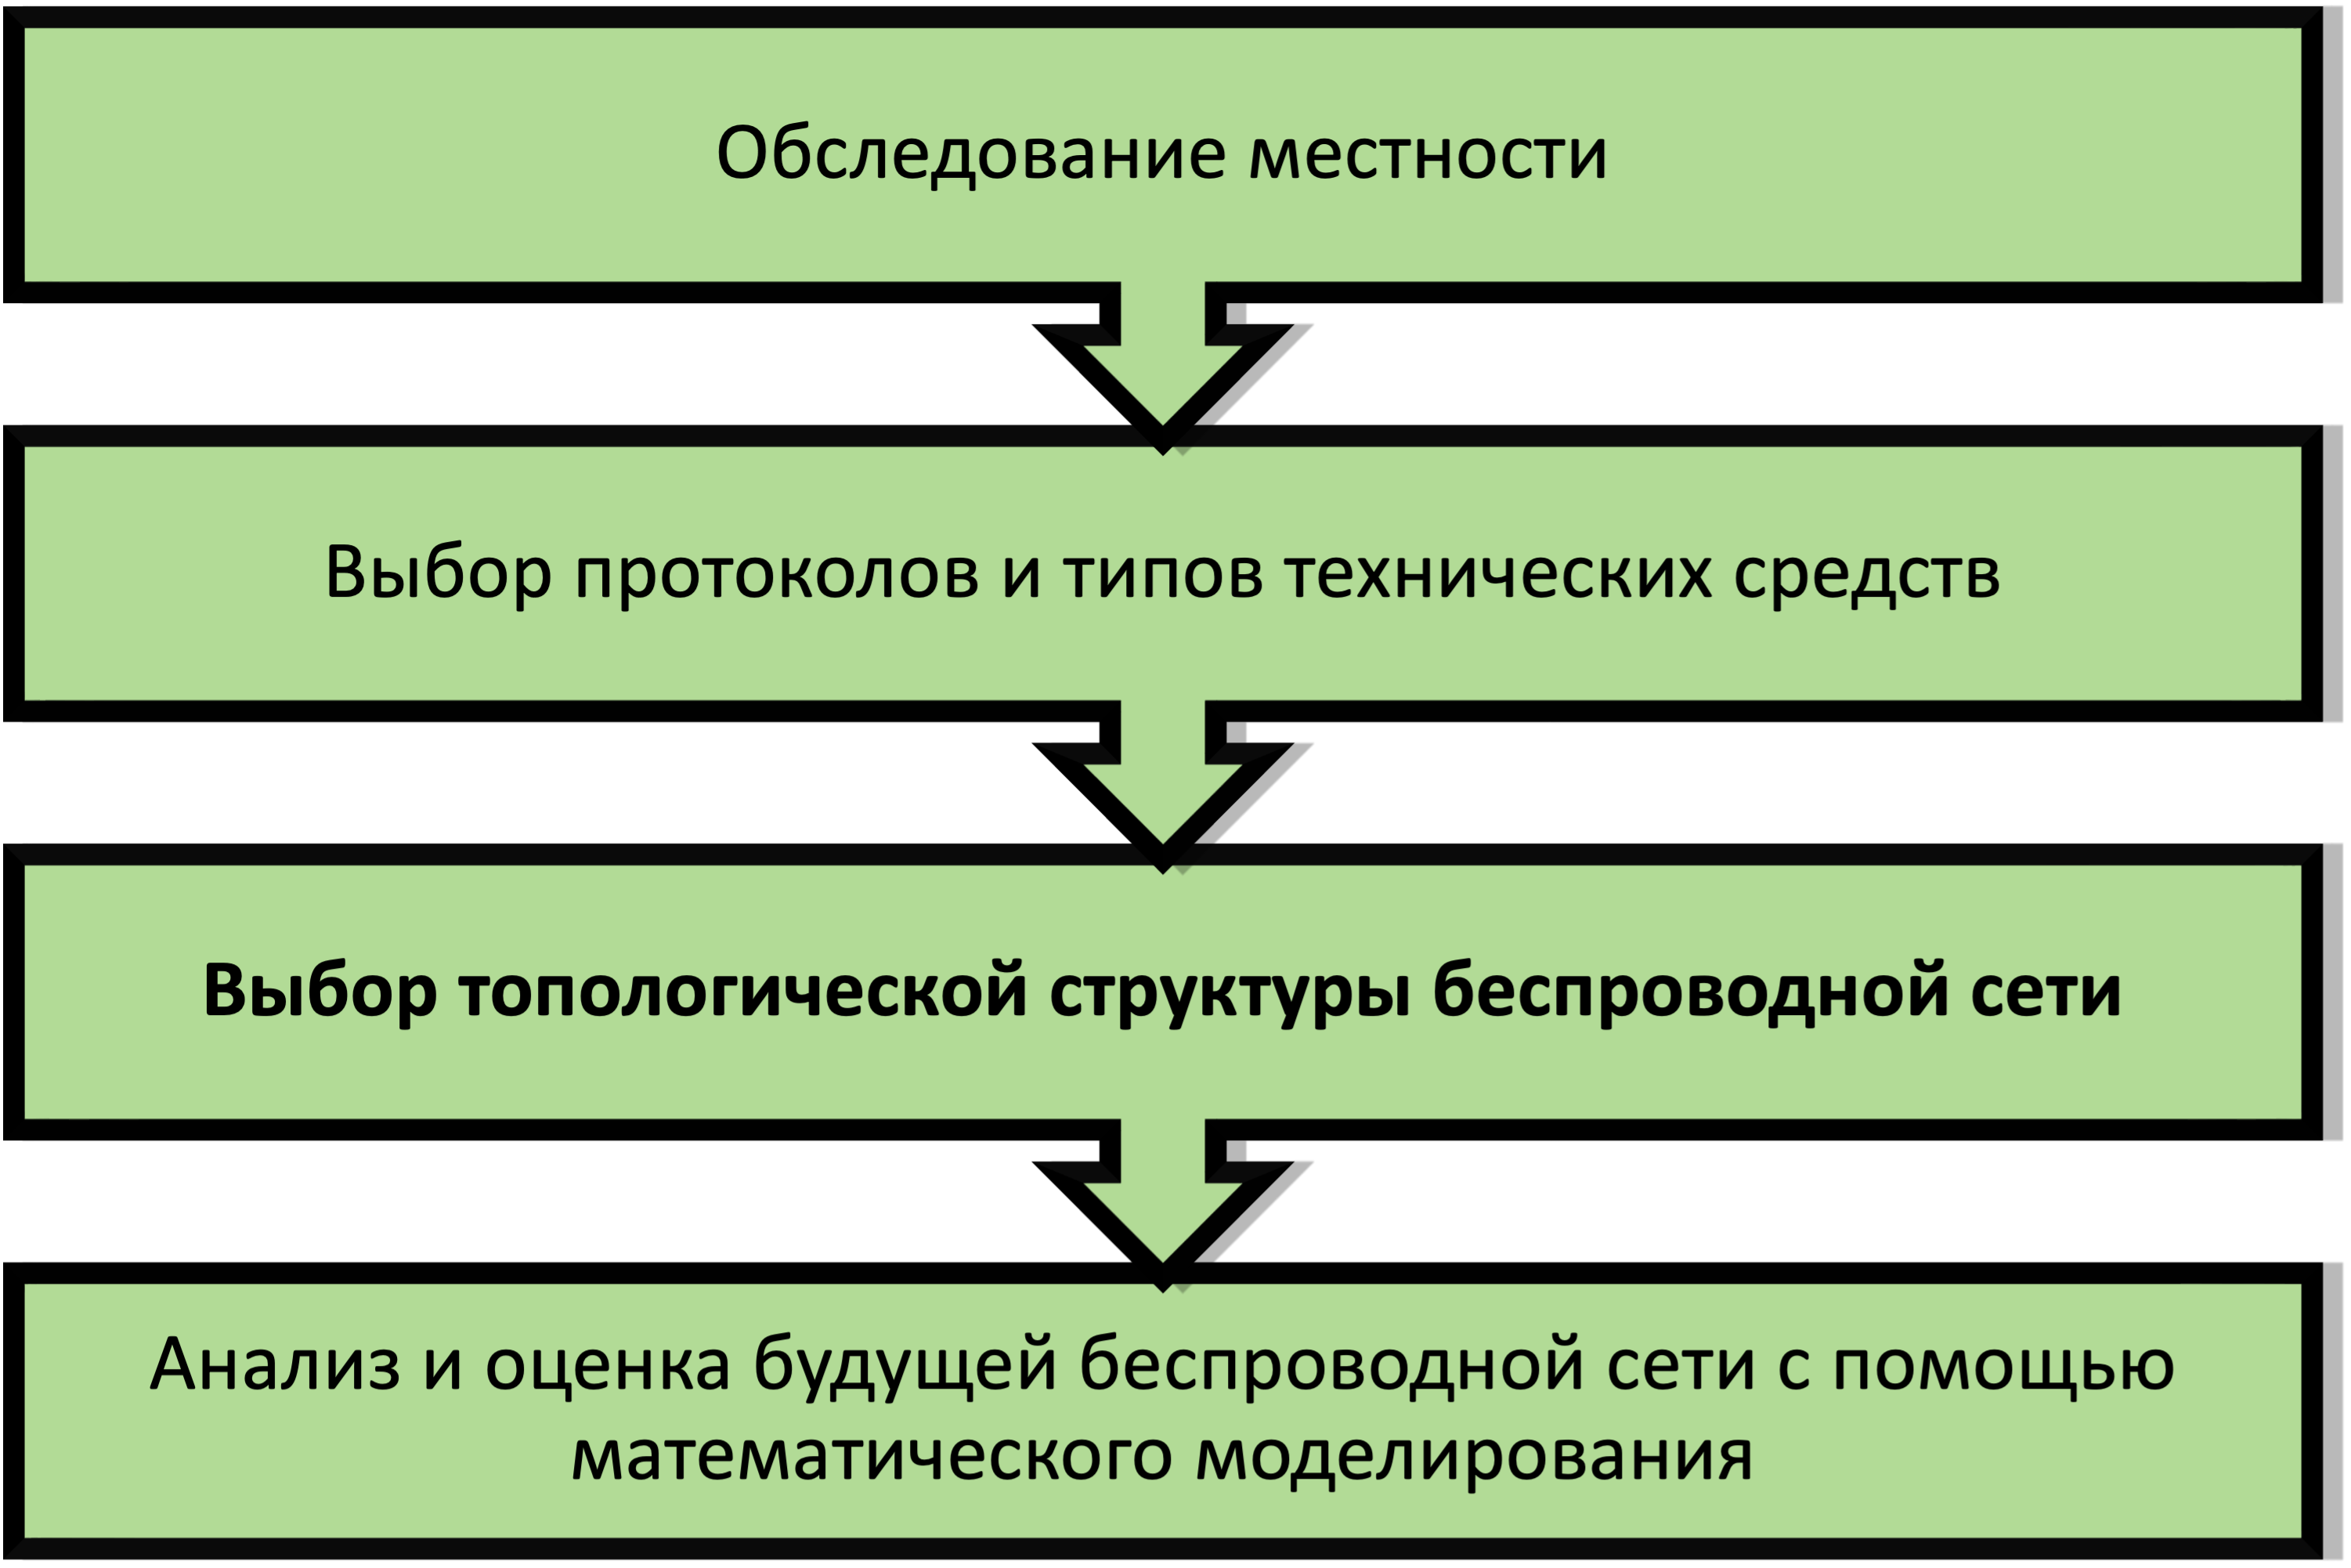
\includegraphics[scale=0.3]{design_stages.png}}


    % \begin{itemize}
    %     \item обследование местности;
    %     \item выбор типов технических средств и протоколов;
    %     \item \textbf{выбор топологической структуры сети;}
    %     \item анализ и оценка производительности сети с помощью математического маделирования.
    % \end{itemize}

    \bigskip
    
    Задача \textbf{синтеза топологии} при комплексном проектировании БШС является основной проблемой исследования в диссертационной работе.

\end{frame}

\begin{frame}
    {Научно-техническая проблема}

    \textbf{\underline{Объектом исследования}} являются БШС специальных типов, широко представленных на практике:
    
    \bigskip

    \begin{itemize}
        \item БШС вдоль протяженных транспортных магистралей;
        \item БШС с ячеистой топологией (mesh) для телекоммуникационного покрытия объектов, рассредоточенных на заданной территории.
    \end{itemize}

    \bigskip

    \textbf{\underline{Предметом исследования}} является синтез топологической структуры беспроводной широкополосной сети.

    \bigskip
    
    \textbf{\underline{Цель диссертационного исследования}} состоит в разработке моделей и методов оптимального размещения базовых станций для беспроводных широкополосных сетей, определяющих топологию таких сетей.

\end{frame}
\note{являются сети специальных типов, широко представленных на практике: беспроводные широкополосные сети вдоль сети вдоль протяженных транспортных магистралей и беспроводные широкополосные сети с ячеистой топологией (mesh) для телекоммуникационного покрытия объектов, рассредоточенных на заданной территории.}

% \section{Положение 1, 2, 3}
\begin{frame}
    \justifying
    \begin{center}
        \fontsize{8pt}{7.2}\selectfont
        {\textbf{Положение 1} - формулировка задачи оптимального размещения базовых станций при проектировании беспроводных широкополосных сетей (БШС) вдоль протяженных транспортных магистралей в виде целочисленного линейного программирования (ЦЛП) и в виде комбинаторной модели в экстремальной форме;}
        \bigskip
        
        {\textbf{Положение 2} - специальный алгоритм типа ветвей и границ для решения сформулированной экстремальной комбинаторной задачи;}
        \bigskip

        {\textbf{Положение 3} - итерационная процедура нахождения последовательности лучших решений для задачи размещения базовых станций в рамках комплексного проектирования БШС вдоль протяженных транспортных магистралей.}
    \end{center}

    \begin{minipage}[t]{0.5\linewidth} 
        
        \center{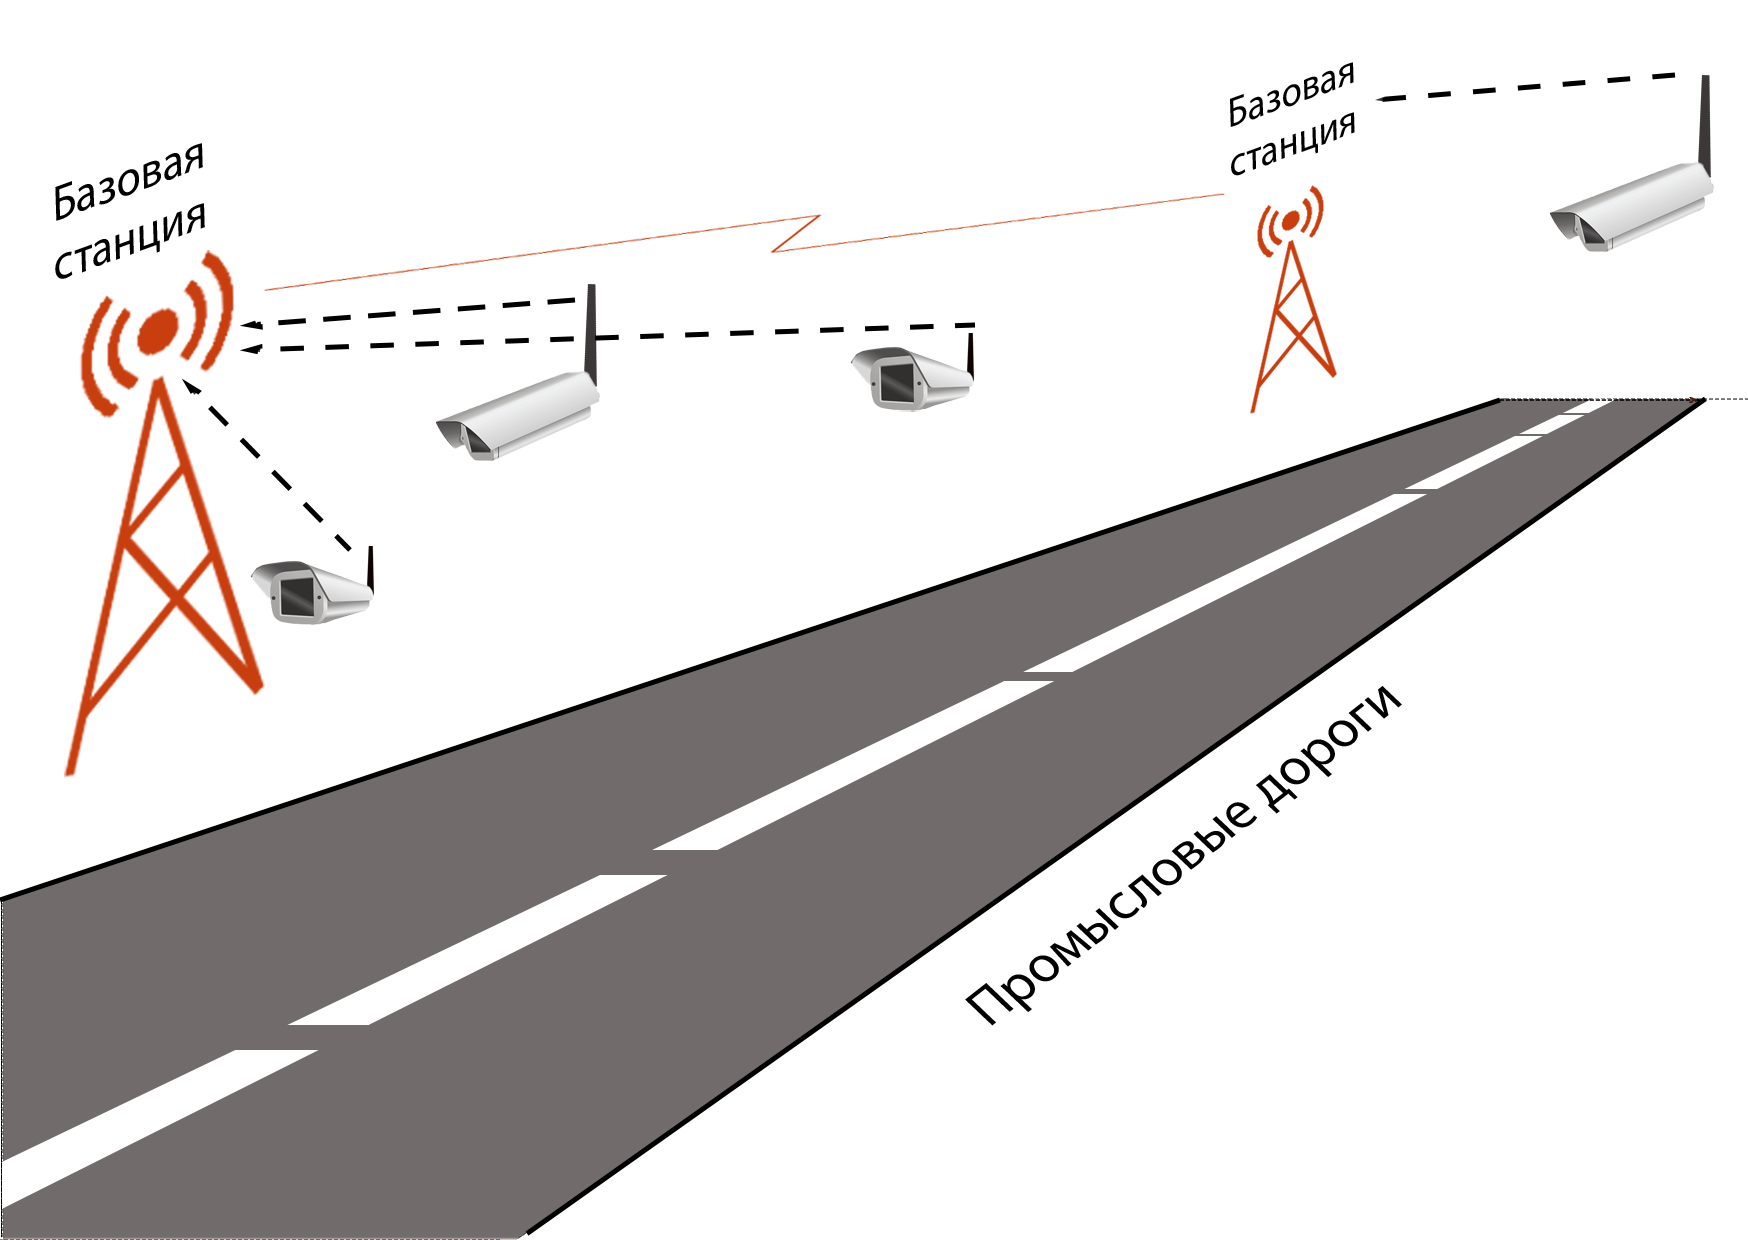
\includegraphics[scale=0.29]{roadsideunit.png}}
        \center{\textbf{Автомобильные дороги}}
    \end{minipage}
    \hfill
    \begin{minipage}[t]{0.4\linewidth}
        \center{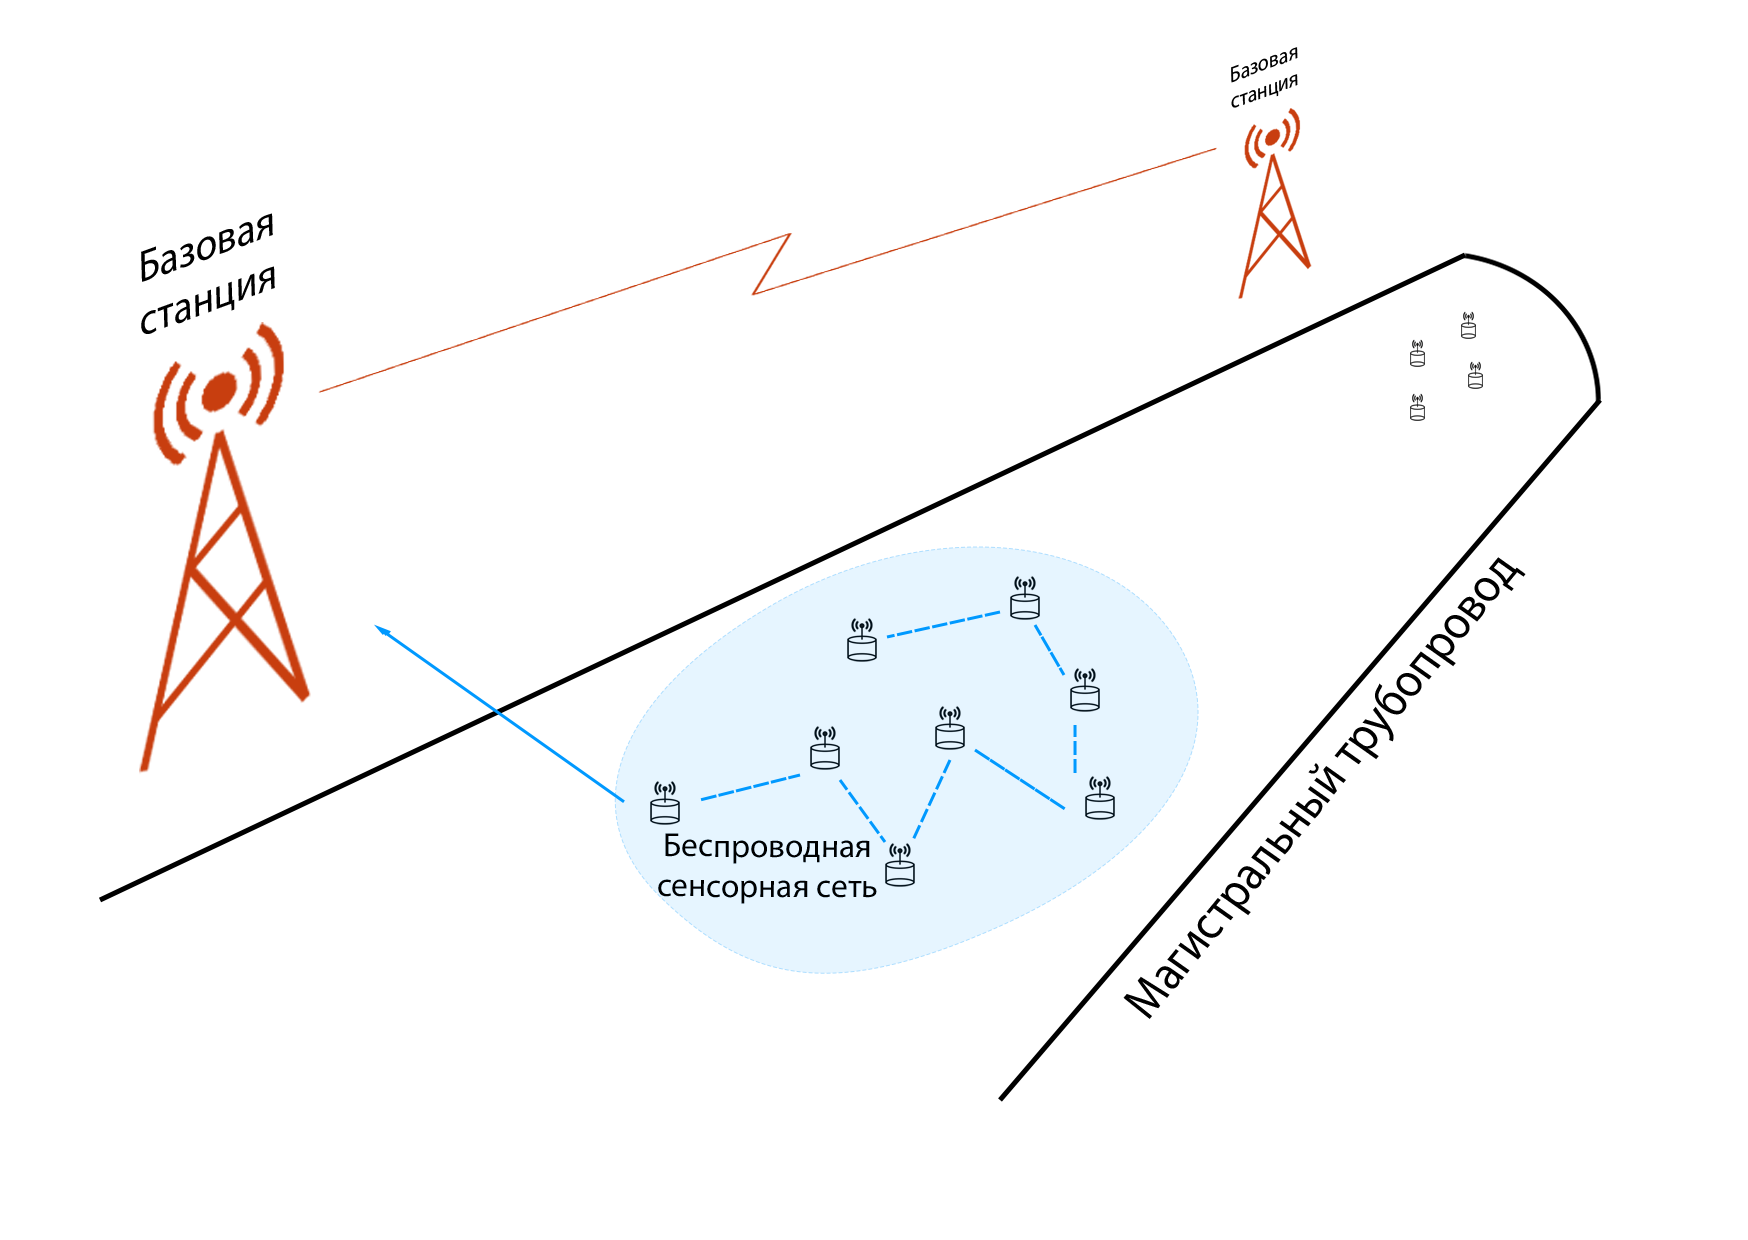
\includegraphics[scale=0.29]{pipeline.png}}
        \center{\textbf{Магистральные и промысловые трубопроводы}}
    \end{minipage}

\end{frame}

\begin{frame}
    {Технологическая постановка задачи} 
    \justifying
    
    Для обеспечения телекоммуникационной связью заданного участка вдоль протяженной транспортной магистрали необходимо разместить базовые приемопередающие устройства (базовые станции) таким образом, чтобы максимизировать телекоммуникационное покрытие с обеспечением условий технических и бюджетных ограничений. 

    \bigskip
    
    Постановки:
    \begin{itemize}
        \item в виде модели ЦЛП;
        \item в виде комбинаторной модели в экстремальной форме.
    \end{itemize}

\end{frame}

% \begin{frame}
%     Важно обеспечить связь любой станции со шлюзами на концах участка через систему размещенных станций. Задано множество станций
% \end{frame}

\begin{frame}
    {задача ЦЛП}
    \justifying
    Задано множество базовых станций (БС) $S = \{s_j\}$. Каждой БС приписаны параметры $s_j = \{r_j, \{R_{jq}\}, c_j \}$, $j = \overline{1,m}; q = \overline{1,m}; q \neq j$. 
    \begin{itemize}
        \item $r_j$ -- радиус телекоммуникационного покрытия БС,
        \item $\{R_{jq} \}$ -- матрица радиусов телекоммуникационной связи между $j$-ой и $q$-ой БС.
        \item $c_j$ -- стоимость.
    \end{itemize} 
    
    % \medskip

    Задан протяженный участок длиной $L$ с концами в точках $a_0$ и $a_{n+1}$. Внутри  отрезка $[a_0, a_{n+1}]$ задано конечное множество точек $A=\{a_i\}, i=\overline{1,n}$; эти точки соответствуют набору свободных мест, где могут быть размещены БС. Каждая точка $a_i$ определяется своей одномерной координатой $l_i$. 
    
    \medskip
    
    Заданы БС специального вида $s_{m+1}$ -- шлюзы. Данные шлюзы размещены на концах $a_0$ и $a_{n+1}$ линейного участка. 
    \bigskip

    \textbf{Требуется} разместить  БС таким образом, чтобы обеспечить связь между шлюзами на концах участка и максимизировать область телекоммуникационного покрытия с условием ограничения на суммарную стоимость $C$.

\end{frame}

% todo: Может быть убрать слайд с расчетом дальности действия телекоммуникационной связи.

% \begin{frame}
%     {задача ЦЛП}
%     \begin{minipage}[t]{1\linewidth}
%         \fontsize{8pt}{7.2}\selectfont
%         \justifying
%         Для расчета параметров радиуса телекоммуникационного покрытия $r_j$ и радиуса телекоммуникационной связи $R_{jq}$, используется уравнение энергетического потенциала канала связи и модели распространения сигнала в пространстве.

%         \bigskip

%         Уравнение энергетического потенциала канала связи:
%         $$
%         P_{tr} - L_{tr} + G_{tr} - L_{fs} + G_{recv} - L_{recv} = SOM + P_{recv},
%         $$
%         где: $P_{tr}$ -- мощность передатчика, дБм; $L_{tr}$ -- потери сигнала на антенном кабеле и разъемах передающего тракта, дБ; $G_{tr}$ -- усиление антенны передатчика, дБ; $L_{fs}$ -- потери в свободном пространстве, дБ; $G_{recv}$ -- усиление антенны приемника, дБ; $L_{recv}$ -- потери сигнала на антенном кабеле и разъемах приемного тракта, дБ; $SOM$ -- запас на замирание сигнала, дБ; $P_{recv}$ -- чувствительность приемника, дБм.

%         \medskip
%         Формула Фрииса, выраженная в децибеллах:
%         $$
%         \label{eq:part3_L_fs}
%         L_{fs} = 20 \lg{F} + 20\lg{R} - G_{tr} - G_{recv} + K,
%         $$
%         где $F$ -- центральная частота, на котором работает канал связи, $R$ -- расстояние между приемной и передающей антенной и $K$ -- константа, зависящая от размерностей частоты и расстояния.

%         \medskip
%         Параметры $r_j$ и $R_{jq}$ рассчитывается как

%         $$
%         R_{jq} / r_j = 10^{\left(\frac{L_{fs} - 20\lg{F} + G_{tr} + G_{recv} - K}{20}\right)}.
%         $$
%     \end{minipage}

% \end{frame}


\begin{frame}
    \frametitle{задача ЦЛП}
    \begin{minipage}[t]{1\linewidth}
        \fontsize{8pt}{7.2}\selectfont
        Целевая функция:
        \begin{equation}
        f =  \sum\limits_{i=1}^n (y_i^- + y_i^+) \rightarrow max,
        \end{equation}

        где $y_i^+$ и $y_i^-$ , $i= \overline{0,n+1}$ определяют охват телекоммуникационного покрытия (справа и слева, соответственно) БС  в точке $a_i$.
        \bigskip
    \end{minipage}

    \begin{minipage}[t]{0.5\linewidth} 
        \fontsize{8pt}{7.2}\selectfont
        Каждая БС должна быть размещена только в одной точке:
            
        \begin{equation}
        \label{eq:part3_xij}
        \sum\limits_{j=1}^n x_{ij} \leq 1, \quad j = \overline{1,m}. 
        \end{equation}
        
        % Значения покрытий не превышают радиус покрытия станции, размещенной в точке $ a_i $, и равны 0, если в точке $a_i$  нет станции \cref{eq:part3_yi_1, eq:part3_yi_2}:
        
        
        \begin{equation}
        \label{eq:part3_yi_1}
        y_i^+ \leq \sum\limits_{j=1}^m x_{ij} \cdot r_j, \quad i = \overline{1,n};
        \end{equation}
        
        \begin{equation}
        \label{eq:part3_yi_2}
        y_i^- \leq \sum\limits_{j=1}^m x_{ij} \cdot r_j, \quad i = \overline{1,n}. 
        \end{equation}

        $$
            x_{ij} = 
             \begin{cases}
               1& \text{, станция $s_j$, размещенная на точке $a_i$,} \\
               0 & \text{, в противном случае.}
             \end{cases}
        $$

    \end{minipage}
    \hfill
    \begin{minipage}[t]{0.4\linewidth}
        
        \center{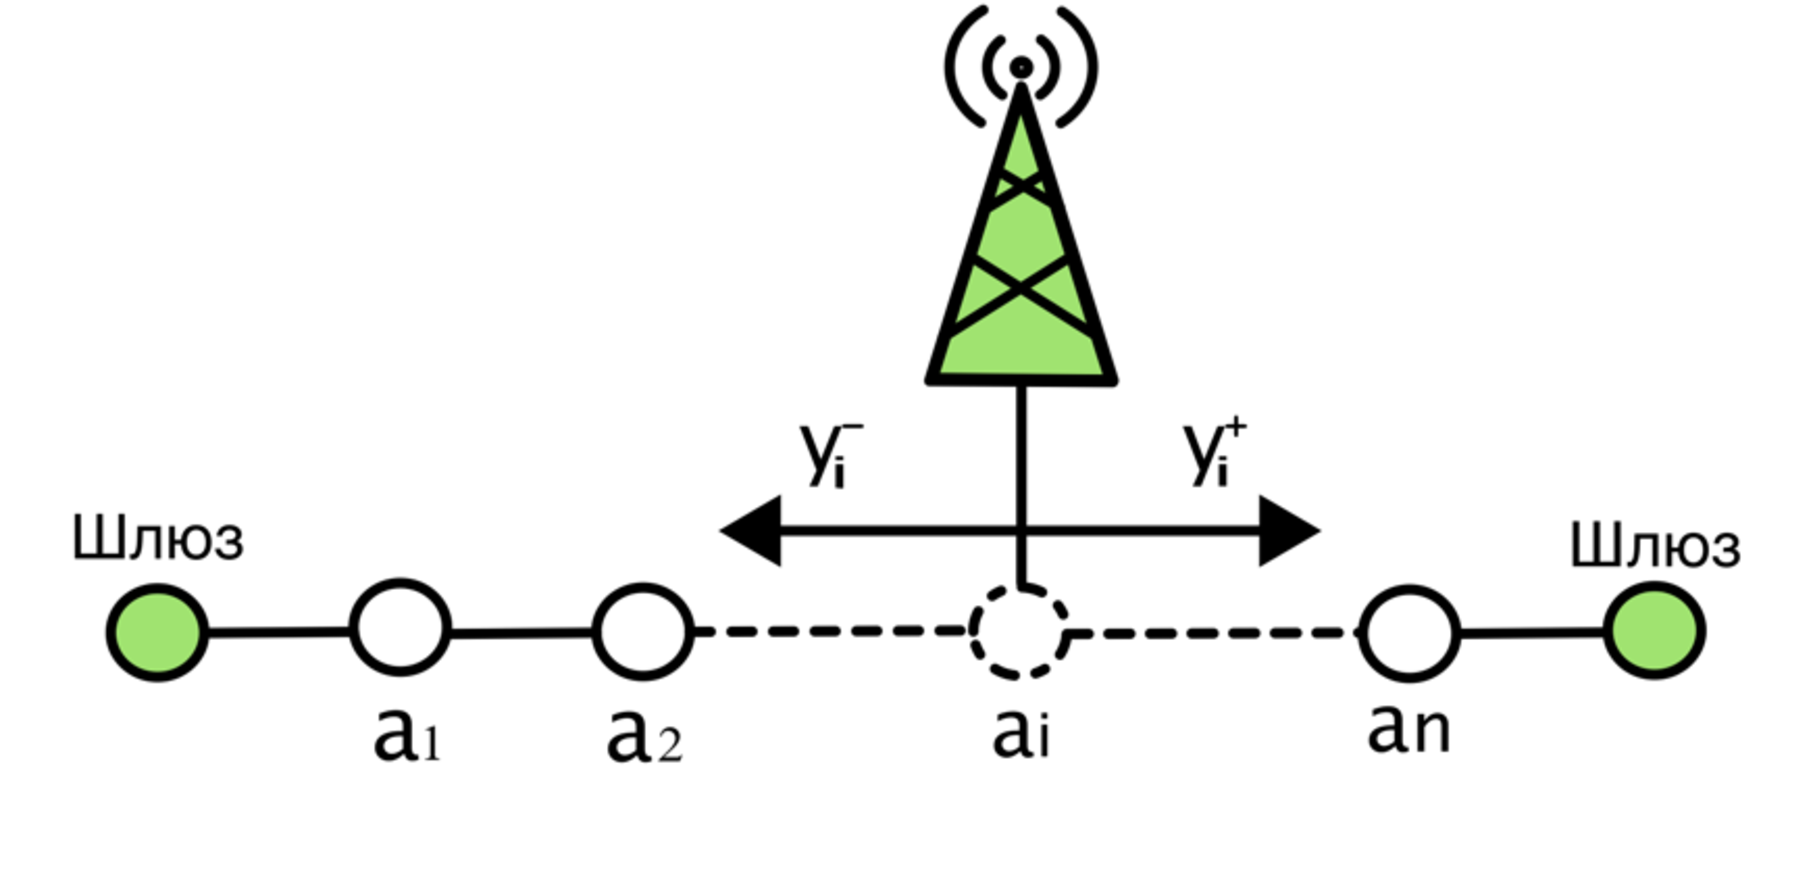
\includegraphics[scale=0.15]{station_coverage.pdf}}
        \center{\textbf{Охват телекоммуникационного покрытия БС}}
    \end{minipage}

    % \bigskip
    % \fontsize{8pt}{7.2}\selectfont
    % где $y_i^+$ и $y_i^-$ , $i= \overline{0,n+1}$ определяют охват покрытия (справа и слева, соответственно) станций.

\end{frame}

\begin{frame}
    \frametitle{задача ЦЛП}
    \fontsize{8pt}{7.2}\selectfont
    \begin{minipage}[t]{0.5\linewidth}
        
    $$
    e_{i} = 
     \begin{cases}
       1& \text{, если какая-либо БС находится в точке $ a_i $} \\
       0 & \text{, в противном случае.}
     \end{cases}
    $$
    \end{minipage}


    \begin{minipage}[t]{0.5\linewidth}
        \begin{equation}
            \label{eq:part3_ei}
            e_i =  \sum\limits_{i=1}^m x_{ij}, \quad i = \overline{1,n}. 
          \end{equation}
    \end{minipage}


    \bigskip

    \begin{minipage}[t]{0.5\linewidth}  
        \fontsize{10pt}{12}\selectfont
        
    
    \bigskip
    \bigskip

    Суммарное телекоммуникационное покрытие между двумя БС не больше расстояния между ними.
          

    \end{minipage}
    \hfill
    \begin{minipage}[t]{0.47\linewidth}
        
        \center{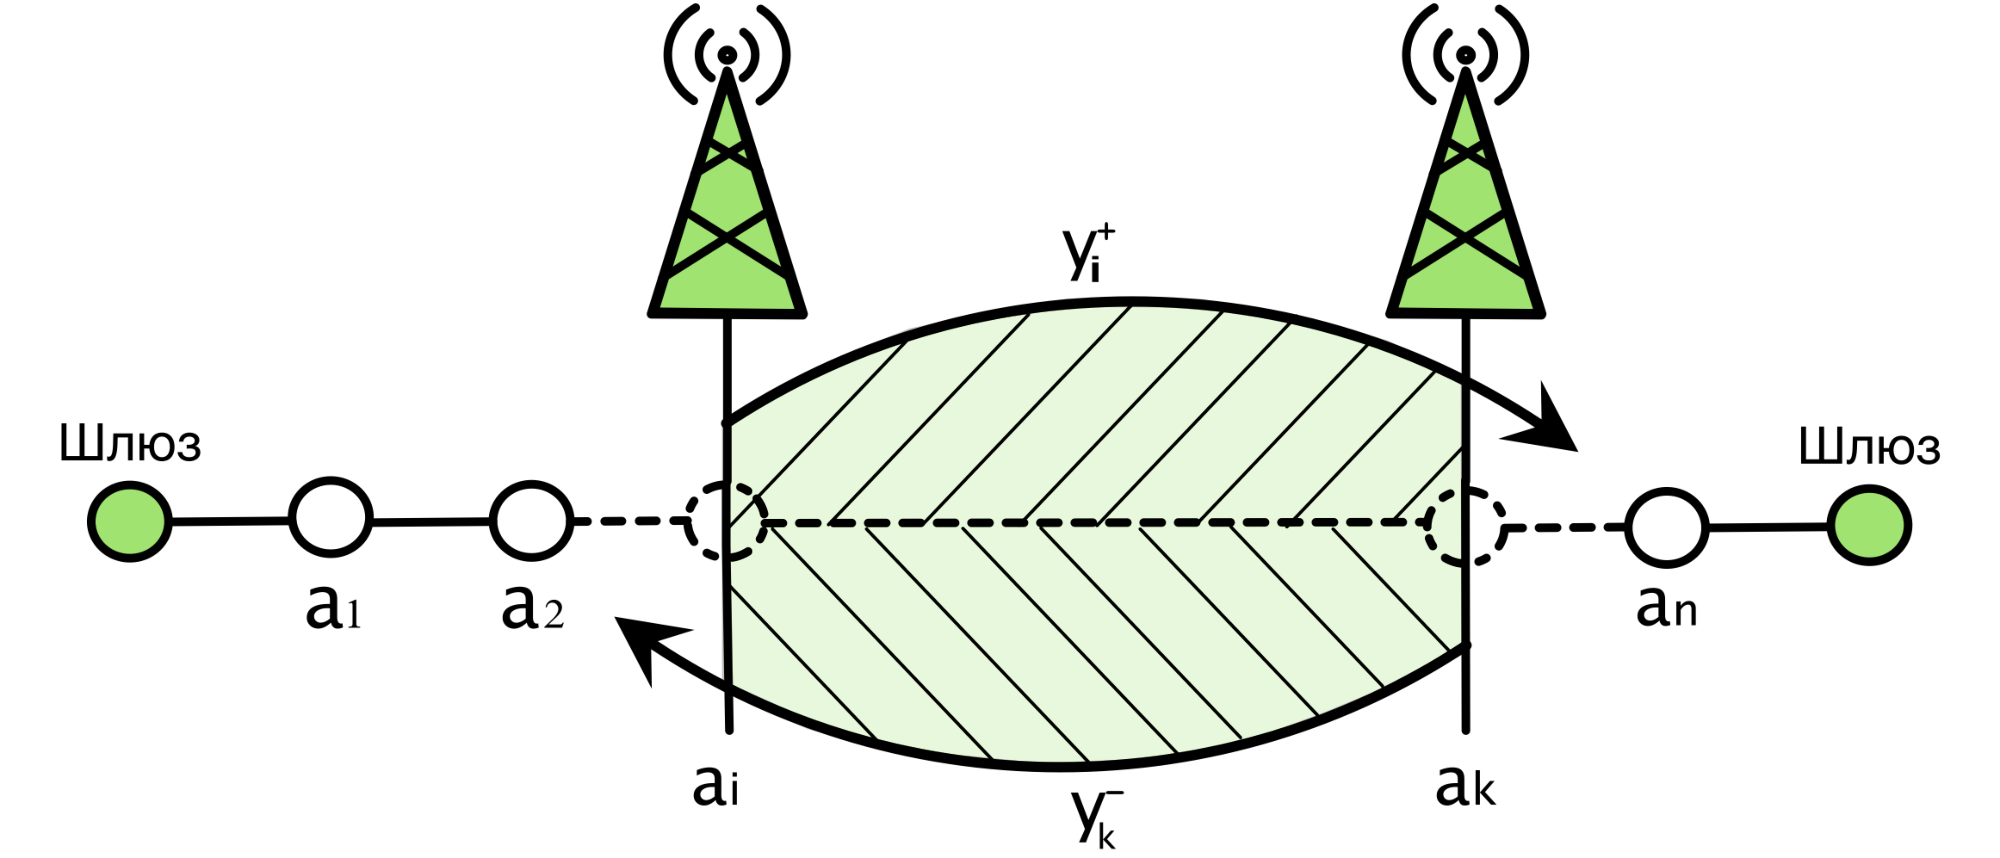
\includegraphics[scale=0.15]{total_coverage_between_points.pdf}}
        \center{\textbf{Телекоммуникационное покрытие между БС}}
    \end{minipage}

    \bigskip
    \fontsize{8pt}{7.2}\selectfont
    \begin{equation}
        \label{eq:part3_yi_3}
        y_i^+ + y_k^- \leq \frac{l_k - l_i}{2} \cdot (e_i + e_k ) + (2 - e_i - e_k ) \cdot L, \quad i = \overline{1,n},  \quad k = \overline{i+1,n+1};
      \end{equation}
      
      \begin{equation}
        \label{eq:part3_yi_4}
        y_i^- + y_k^+  \leq \frac{l_i-l_k}{2} \cdot (e_i + e_k) + (2 - e_i - e_k) \cdot L, \quad i = \overline{1,n}, \quad k = \overline{i-1,0},
      \end{equation}

\end{frame}

\begin{frame}
    \frametitle{задача ЦЛП}
    \begin{minipage}[t]{1\linewidth}
        \fontsize{9pt}{7.2}\selectfont
        Введем переменные $z_{ijkq}, i = \overline{1,n}; j= \overline{1,m}; k=\overline{1,n},  k \neq i; q= \overline{1,m}, q \neq j$.
    \bigskip
    $$
    z_ {ijkq} = 
     \begin{cases}
       1& \text{, если в точке $ a_i $ размещена станция $ s_j $} \\
        & \text{и данная станция связана со станцией} \\
        & \text{$ s_q $, размещенная в точке $ a_k $;} \\
       0 & \text{, в противном случае.}
     \end{cases}
    $$
    \bigskip
    \end{minipage}
    
    \begin{minipage}[b]{0.5\linewidth}
        Важно обеспечить связь любой БС со шлюзами на концах участка через систему размещаемых БС. 

    \end{minipage}
    \hfill
    \begin{minipage}[t]{0.47\linewidth}
        
        \center{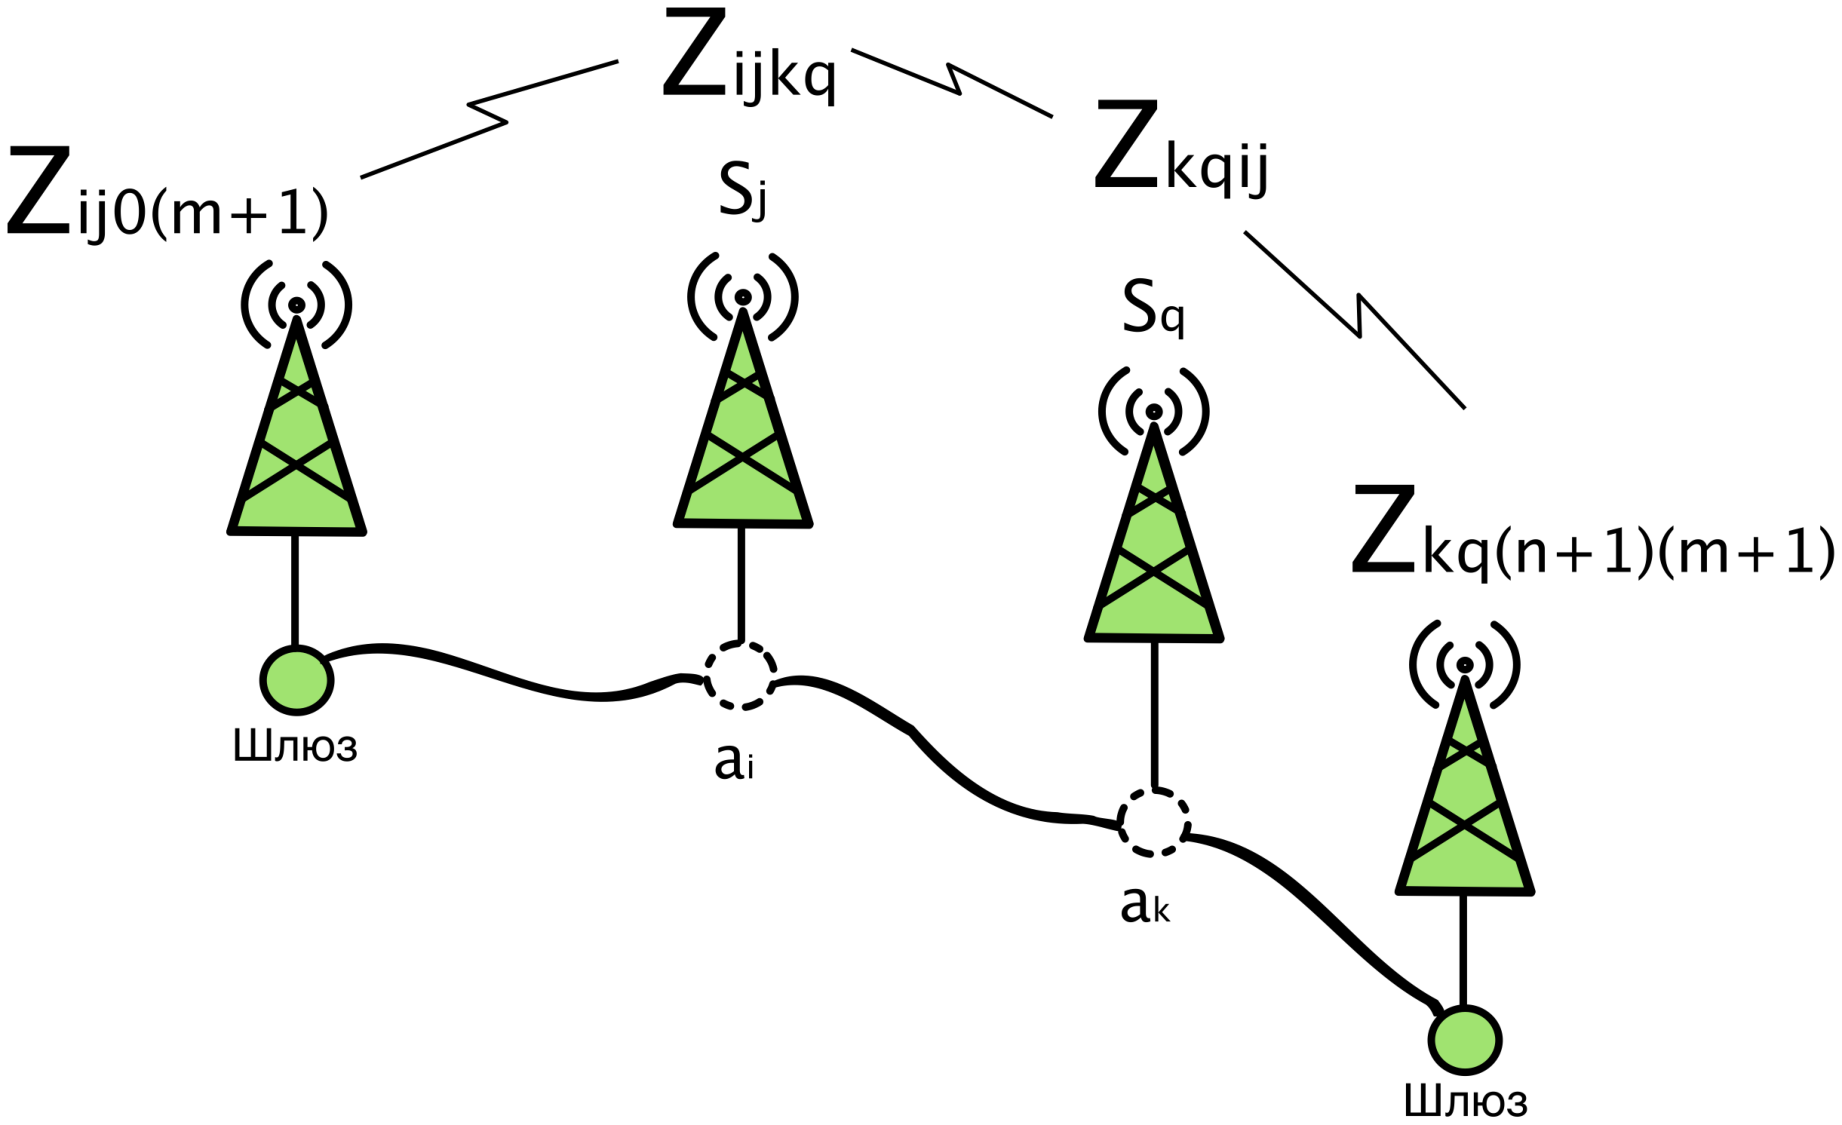
\includegraphics[scale=0.15]{station_link.pdf}}
        \center{\textbf{Связь между станциями}}
    \end{minipage}

\end{frame}

\begin{frame}
    \frametitle{задача ЦЛП}
    
    \begin{minipage}[t]{0.99\linewidth}
        \fontsize{8 pt}{7.2}\selectfont
        \begin{equation}
            \label{eq:part3_z_ijkq_1}
            z_{ijkq} \leq e_i , \quad i = \overline{1, n}; \quad j = \overline{1, m}; \quad k = \overline{1,n}, k \neq i; \quad q = \overline{1,m}, q \neq j;
        \end{equation}
        
        
        \begin{equation}
            \label{eq:part3_z_ijkq_2}
            z_{ijkq} \leq e_k , \quad k = \overline{1, n}; \quad j = \overline{1, m}; \quad i = \overline{1,n}, i \neq k; \quad q = \overline{1,m}, q \neq j.
        \end{equation}
        
        
        \begin{equation}
            \label{eq:part3_z_ijkq_3_1}
            \sum\limits_{k=i+1}^{n} \sum\limits_{\substack{q = 1\\ q \neq j}}^m z_{ijkq} + z_{ij(n+1)(m+1)} = x_{ij} ,  \quad i = \overline{1, n}, \quad j = \overline{1, m}.
        \end{equation}

        \begin{equation}
            \label{eq:part3_z_ijkq_1_2}
            \sum\limits_{k=i+1}^{n} \sum\limits_{\substack{q = 1\\ q \neq j}}^m z_{kqij} + z_{(n+1)(m+1)ij} = x_{ij} ,  \quad i = \overline{1, n}, \quad j = \overline{1, m}.
        \end{equation}

        \begin{equation}
            \label{eq:part3_z_ijkq_2_1}
            z_{ij0(m+1)} + \sum\limits_{k=1}^{i-1} \sum\limits_{\substack{q = 1\\ q \neq j}}^m z_{ijkq}= x_{ij}, \quad i = \overline{1, n}, \quad j = \overline{1, m}.
          \end{equation}
      
          
        \begin{equation}
        \label{eq:part3_z_ijkq_2_2}
            z_{0(m+1)ij} +  \sum\limits_{k=1}^{i-1} \sum\limits_{\substack{q = 1 \\ q \neq j}}^m z_{kqij}= x_{ij},  \quad i = \overline{1, n}, \quad j = \overline{1, m}.
        \end{equation}

     
    \end{minipage}

\end{frame}


% \begin{frame}[plain, noframenumbering]
%     \frametitle{задача ЦЛП}
    
%     \begin{minipage}[t]{0.99\linewidth}
%         \fontsize{8 pt}{7.2}\selectfont
%         \begin{equation}
%             \label{eq:part3_z_ijkq_1}
%             z_{ijkq} \leq e_i , \quad i = \overline{1, n}; \quad j = \overline{1, m}; \quad k = \overline{1,n}, k \neq i; \quad q = \overline{1,m}, q \neq j;
%         \end{equation}
        
        
%         \begin{equation}
%             \label{eq:part3_z_ijkq_2}
%             z_{ijkq} \leq e_k , \quad k = \overline{1, n}; \quad j = \overline{1, m}; \quad i = \overline{1,n}, i \neq k; \quad q = \overline{1,m}, q \neq j.
%         \end{equation}
        
        
%         \begin{equation}
%             \label{eq:part3_z_ijkq_3_1}
%             \sum\limits_{k=i+1}^{n} \sum\limits_{\substack{q = 1\\ q \neq j}}^m z_{ijkq} + z_{ij(n+1)(m+1)} = x_{ij} ,  \quad i = \overline{1, n}, \quad j = \overline{1, m}.
%         \end{equation}

        
%         \begin{equation}
%             \label{eq:part3_z_ijkq_3_2}
%             z_{nj(n+1)(m+1)} = x_{nj} \quad j = \overline{1, m}.
%         \end{equation}

        
%         \begin{equation}
%             \label{eq:part3_z_ijkq_4_1}
%             z_{1j0(m+1)}= x_{ij}, \quad j = \overline{1, m};
%         \end{equation}

        
%         \begin{equation}
%             \label{eq:part3_z_ijkq_4_2}
%             z_{ij0(m+1)} + \sum\limits_{k=1}^{i-1} \sum\limits_{\substack{q = 1\\ q \neq j}} z_{ijkq}= x_{ij}, \quad i = \overline{2, n}, \quad j = \overline{1, m}.
%         \end{equation}

        
%         \begin{equation}
%             \label{eq:part3_z_ijkq_5}
%             \sum\limits_{i=k+1}^{n} \sum\limits_{\substack{j=1 \\ j \neq q}}^m z_{ijkq} = x_{kq} , \quad k = \overline{1, n-1}, \quad q = \overline{1, m};
%         \end{equation}

        
%         \begin{equation}
%             \label{eq:part3_z_ijkq_6}
%             \sum\limits_{i=1}^{k} \sum\limits_{\substack{j=1 \\ j \neq q}}^m z_{ijkq} = x_{kq} , \quad k = \overline{2, n}, \quad q = \overline{1, m};
%         \end{equation}
%     \end{minipage}
% \fixme{Check confitions It's wrong!}
% \end{frame}


\begin{frame}
    \frametitle{задача ЦЛП}
    \begin{minipage}[t]{1\linewidth}
        \fontsize{6pt}{7.2}\selectfont
        $\forall i= \overline{1,n}$:
        \begin{equation}
          \label{eq:part3_z_ijkq_7}
          z_{ijkq}(R_{jq}-(a_i-a_k )) \geq 0, \quad k=\overline{0,i-1}; \quad j=\overline{1,m}; \quad q= \overline{1,m}, q \neq j; 
        \end{equation}
        
        \begin{equation}
          \label{eq:part3_z_ijkq_8}
          z_{ijkq} (R_{qj}-(a_k-a_i )) \geq 0, \quad k=\overline{i+1,n+1}; \quad j=\overline{1,m}; \quad q= \overline{1,m}, q \neq j.
        \end{equation}
    \medskip
    \end{minipage}
    
    \begin{minipage}[и]{0.5\linewidth}
        \fontsize{7pt}{7.2}\selectfont
        Радиусы телекоммуникационной связи размещаемых БС должны быть не меньше расстояния между ними
        \bigskip
        % \bigskip
        % \bigskip

    \end{minipage}
    \hfill
    \begin{minipage}[b]{0.47\linewidth}
        
        \center{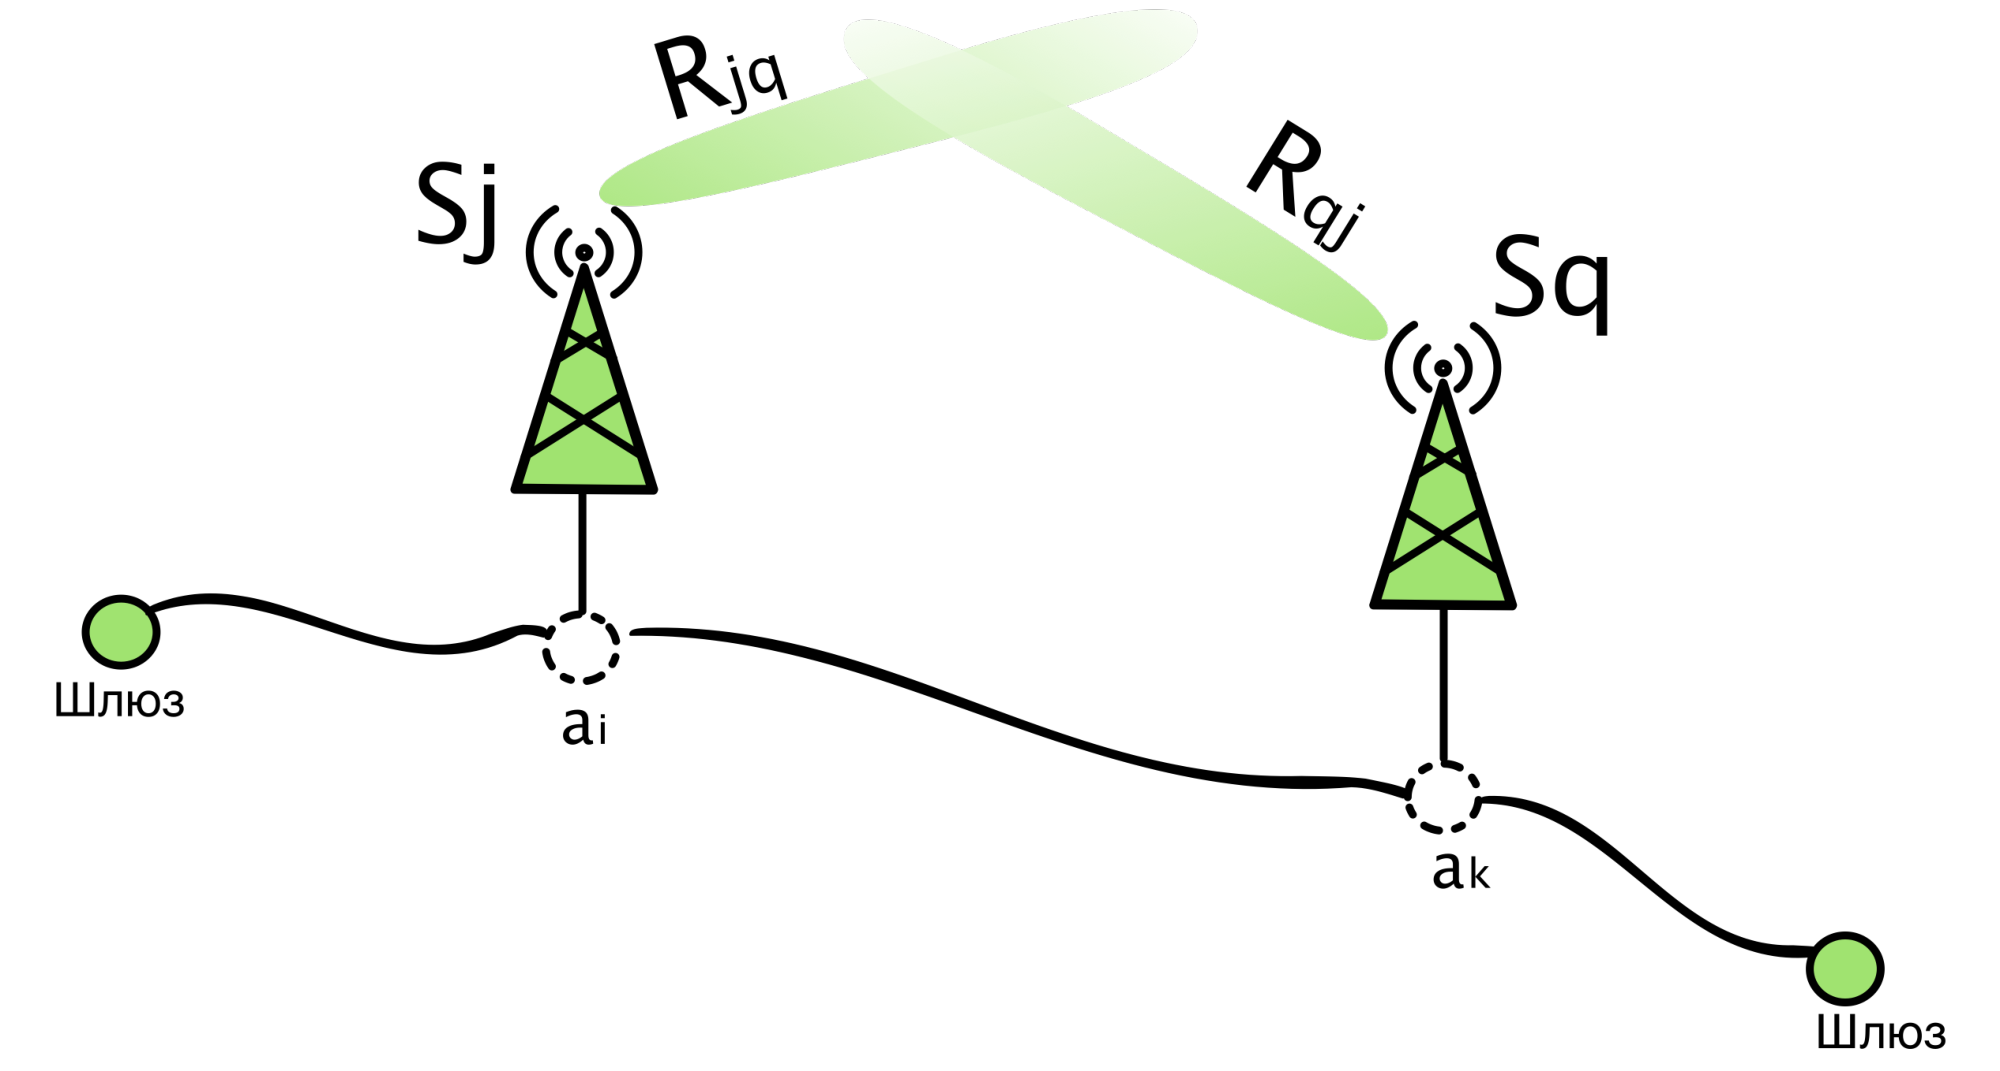
\includegraphics[scale=0.1]{station_link_between_points.pdf}}
        \center{\textbf{Обеспечение телекоммуникационной связью с соседней БС}}
    \end{minipage}
    % \hfill
    \begin{minipage}[b]{0.99\linewidth}
        \fontsize{7pt}{7.2}\selectfont
        И бюджетное ограничение:

        \begin{equation}
        \label{eq:part3_cost}
        \sum\limits_{i=1}^n \sum\limits_{j=1}^m x_{ij} \cdot c_j \leq C,
        \end{equation}
        где $c_j$ -- стоимость БС $s_j$.
    \end{minipage}

\end{frame}

\begin{frame}
    \frametitle{задача ЦЛП}
    \justifying
    
    Работа$^1$ содержит доказательство NP-трудности для частного случая задачи ЦЛП, когда вдоль транспортной магистрали размещают множество однотипных БС с одинаковыми параметрами. 
    \bigskip
    
    Представленная в исследовании модель (1) - (16) рассматривает общий случай размещения, когда вдоль транспортной магистрали размещают множество различных БС с разными техническими параметрами. Следовательно, данная задача является также NP-трудной.
    \bigskip

    % Представленная математическая модель рассчитывалась в пакете 
    
    % Optimization Toolbox MATLAB.
    % Представленная математическая модель рассчитывалась алгоритмом Лэнд и Дойг (1960).
    \bigskip

    \bigskip
    \bigskip
    \begin{minipage}[b]{0.99\linewidth}
        \fontsize{6pt}{7.2}\selectfont
    \textit{1. On a problem of base stations optimal placement in wirelessnetworks with linear topology. — [текст]. / — R. Ivanov [и др.] //Communications in Computer and Information Science. — 2018. —т. 919. — с. 505—513.}
    \end{minipage}

\end{frame}

\begin{frame}
    \frametitle{Комбинаторная модель}
    \justifying
    Модели ЦЛП не учитывает:
    \begin{itemize}
        \item алгоритмы решения общего вида задач ЦЛП не учитывают специфику конкретной задачи.
        \item ограничение на величину межконцевой задержки сети, ее невозможно привести к линейному виду;
    \end{itemize}
    

    \medskip
    Разработан специальный алгоритм размещения базовых станций на основе \textbf{метода ветвей и границ (МВиГ)} для комбинаторной модели в экстремальной форме.

    \medskip

    Задано множество станций $S = \{s_j\}$, $s_j=\{r_j,\{R_{jq} \},p_j, c_j \}$, $j=1,...,m;q=1,...,m;j \neq q $, где 
    \begin{itemize}
        \item $r_j$ -- радиус покрытия БС,
        \item $R_{jq}$ -- радиус телекоммуникационной связи между БС $s_j$ и $s_q$,
        \item \textbf{$p_j$ -- пропускная способность},
        \item $c_j$ -- стоимость;
    \end{itemize} 

    % \bigskip
    % \textit{Допустимой расстановкой станций} назовем такой возрастающий по величине координат $l_i$  набор пар $P = \{a_i, s_j\},a_i \in A,i \neq 0,i \neq n+1;s_j \in S$.
    \medskip
    \textbf{Требуется} разместить БС таким образом, чтобы максимизировать область телекоммуникационного покрытия отрезка $L$ с учетом ограничений на величину межконцевой задержки $T$ и суммарную стоимость размещения $C$.


\end{frame}


\begin{frame}
    \justifying
    \frametitle{Оценка межконцевой задержки}
    \fontsize{8pt}{7.2}\selectfont

    Одним из ограничений для алгоритма МВиГ является межконцевая задержка сети $T$.
    \bigskip

    Для оценки характеристики используют стохастические модели сетей массового обслуживания.
    \center{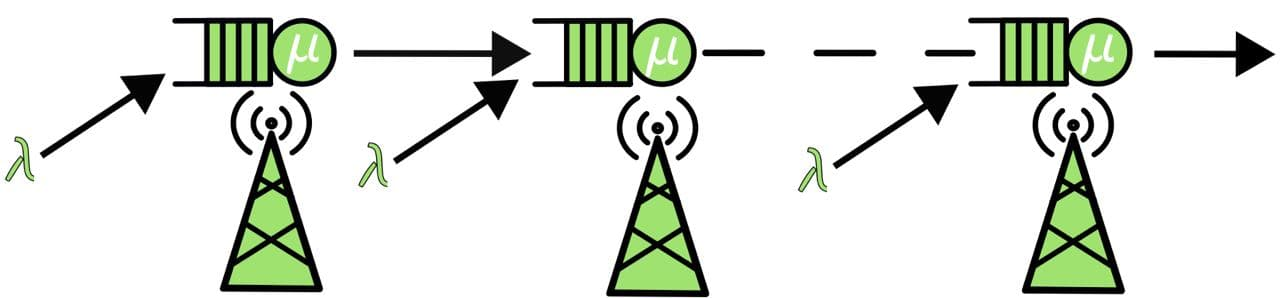
\includegraphics[scale=0.2]{tandem_queue.png}}
    \center{\textbf{Многофазная сеть массового обслуживания}}

    \bigskip

    {Рассмотрим сеть как модель многофазной сети массового обслуживания  с узлами $M/M/1$, с линейной топологией, с $N$ последовательно соединенными узлами и кросс-трафиком. 

    \bigskip
    % В такой системе  интервалы между поступлениями пакетов задается случайной величиной $A \sim Exp(\lambda)$ и время обслуживания с помощью случайной величины $S \sim Exp(\mu)$.

    В такой системе $M$ -- интервалы между поступлениями пакетов задается экспоненциальным распределением; $M$ --  время обслуживания задается экспоненциальным распределением; 1 -- в каждом узле одно обслуживающее устройство.}

   
\end{frame}

% todo: T для M/M/1 (может вернуть)

% \begin{frame}
%     \justifying
%     \frametitle{Оценка межконцевой задержки}
%     \fontsize{8pt}{7.2}\selectfont

%     На каждый узел входящие потоки поступают с интесивностью $\lambda$. 

%     По теореме Бурке на выходе узла $M/M/1$, а значит на входе каждой последующей фазы тоже пуассоновский поток с интенсивностью $\lambda$.
    
%     \bigskip

%     По формуле Литтла можно рассчитать время задержки на фазе. 

%     \begin{displaymath}
%         \mu_j = p_j / w,
%     \end{displaymath}
%     где $p_j$ - пропускная спобоcтность $j$-ой станции, Мбит/с; $w$ - средний размер пакета, Мбит.

%     Для каждой станции коэффициент загрузки равен:


%     \begin{displaymath}
%     \rho_j= \frac{\sum{\lambda}}{\mu_j} = \frac{q \cdot \lambda}{\mu_j} <1,
%     \end{displaymath}
%     где $q$ -- число входящих потоков. Условие $\rho_j<1$ является необходимым и достаточным условием существования стационарного режима функционирования СеМО.
    
%     \bigskip
    
%     Тогда среднее время задержки по времени на каждой станции:

%     \begin{displaymath}
%         \overline{T_j} = \frac{\rho_j}{1 - \rho_j} \cdot \frac{1}{q \cdot \lambda}.
%     \end{displaymath}

%     \bigskip

%     Межконцевая задержки в сети равна

%     \begin{equation}
%         \label{eq:end_to_end_delay}
%         T^{e2e}= \sum{\overline{T_j}}.
%     \end{equation}

% \end{frame}

\begin{frame}
    \justifying
    \frametitle{Оценка межконцевой задержки}
    \fontsize{8pt}{7.2}\selectfont

    Было исследованы различные стохастические модели многофазной сети массового обслуживания (СеМО) с кросс-трафиком и узлами: $M/M/1/N$ (экспоненциальным распределением времени обслуживания) и $M/PH/1/N$ (фазовым распределением времени обслуживания), для которых нет точного аналитического расчета.

    \center{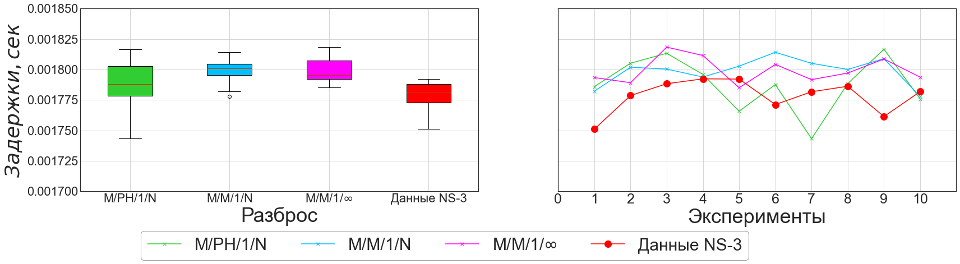
\includegraphics[scale=0.3]{comparison_queue_models.png}}
    \center{\textbf{Сравнение моделей массового обслуживания с данным NS-3}}

    \bigskip
    Модели сравнивались с временными задержками, полученными с помощью имитационного моделирования в среде NS-3 для БШС протокола IEEE 802.11n.

\end{frame}

\begin{frame}
    \justifying
    \frametitle{Оценка межконцевой задержки}
    \fontsize{8pt}{7.2}\selectfont

    Были исследованы прогнозные модели оценок межконцевых задержек для СеМО с узлами $M/M/1$, в которой размер пакетов фиксируется при их первом появлении в имитационной модели и не изменяется в течение всего времени обслуживания на фазах. Данное условие нарушает важное допущение о независимости обслуживания заявок на фазах сети.

    \center{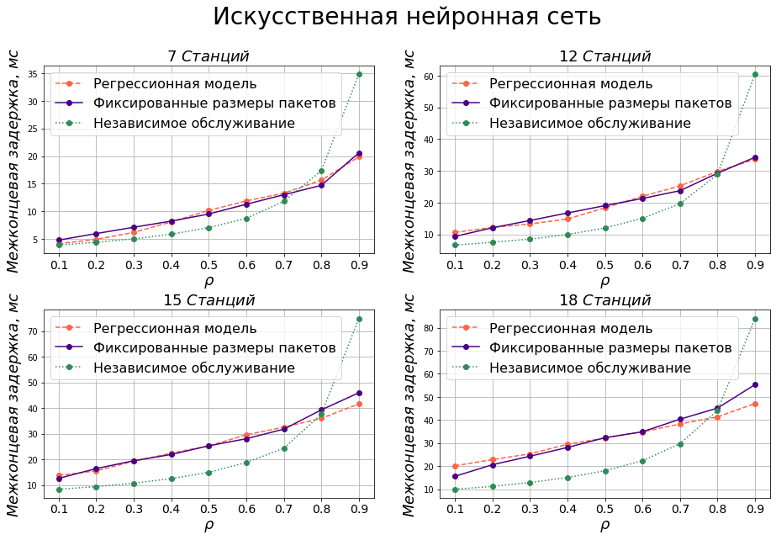
\includegraphics[scale=0.3]{e2e_delay_ml.png}}
    \center{\textbf{Прогнозная модель величины межконцевой задержки для СеМО с зависимым обслуживанием}}


\end{frame}

\begin{frame}
    \justifying
    \frametitle{Оценка межконцевой задержки}
    \fontsize{8pt}{7.2}\selectfont

    С учетом быстрого аналитического решения и достаточного приближения для оценки величины межконцевой задержки в ходе поиска оптимального размещения БС БШС было решено в работе использовать СеМО с узлами $M/M/1$ и кросс-трафиком.

    \bigskip
    В дальнейшем полученную БШС, после этапа синтеза топологии, можно проверять на более сложных моделях. На следующем шаге -- на этапе математического моделирования более основательно проводится оценка характеристик производительности как время задержек, длины очередей, пропускная способность, вероятность потери пакетов и т.д. Такой подход проектирования позволяет провести комплексную проверку соответствия QoS для полученного размещения БС. 
    
    \bigskip
    % На этапе синтеза топологической структуры будет проводиться расчет с помощью быстрой модели для отсева вариантов размещения БС с большими задержками.


\end{frame}

\begin{frame}
    \frametitle{Комбинаторная модель}
    \justifying
    \textbf{Допустимой расстановкой} базовых станций назовем такой возрастающий по величине координат $l_i$  набор пар $P = \{a_i, s_j\},a_i \in A,i \neq 0,i \neq n+1;s_j \in S$.

    Для каждой расстановки выполняются \textbf{требования}:

    \begin{enumerate}
        \item  для каждой пары $(a_i,s_j)$:
            \begin{itemize}
                \item слева: либо найдется такая пара $(a_k,s_q)$, что, $l_i - l_k \leqslant R_{jq}$  и $l_i - l_k  \leqslant R_{qj}$, либо $l_i-l_0 \leqslant R_{j0}$ и $l_i - l_0 \leqslant R_{0j}$;
                \item справа: либо найдется такая пара $(a_t,s_g)$, что, $l_t-l_i \leqslant R_{jq}$ и $l_t - l_i \leqslant R_{qj}$, либо $l_{n+1}-l_i \leqslant R_{j(m+1)}$ и $l_{n+1}-l_i \leqslant R_{(m+1)j}$. 
            \end{itemize}
    Данное требование гарантирует, что любая БС может быть связана со шлюзами на концах отрезка либо через промежуточные БС, либо непосредственно, если таковых нет;
        \item суммарная стоимость размещенных БС меньше заданного ограничения  $C$.
        \item суммарная задержка по всем размещенным БС меньше заданной величины $T$ –- средней межконцевой задержки по времени;
    \end{enumerate}

\end{frame}

\begin{frame}
    \frametitle{Комбинаторная модель}
    \justifying
    Каждой допустимой расстановке БС $P$ соответствует величина телекоммуникационного покрытия $z(P)$, определяемая как суммарная область покрытия БС, входящих в набор пар $P$.

    Для удобства описания в дальнейшем алгоритмов введем понятие <<недопокрытия>> $f(P)$:

    \begin{displaymath}
        f(P) = L - z(P)
    \end{displaymath} 

    \textbf{Задача 1.}
    Пусть $G$ -- множество всех допустимых расстановок $P$.

    \bigskip

    Тогда требуется найти такую расстановку  $P^*$, что
    \begin{displaymath}
        \label{eq:present_P}
        P^* = \argmin \limits_{P \in G} f(P)
    \end{displaymath}
\end{frame}

\begin{frame}
    \frametitle{Комбинаторная модель}
    \justifying
    \begin{minipage}[t]{1\linewidth}
        \fontsize{8pt}{7.2}\selectfont
        \textbf{Процедура построения бинарного дерева поиска} 
        \bigskip

        На каждой итерации, начиная с итерации $\nu=0$, разбиваем текущее подмножество $G_\nu$ на два подмножества $G^1_\nu$ и $G^2_\nu$. 
    \bigskip
    \end{minipage}
    
    \begin{minipage}[b]{0.5\linewidth}
        \fontsize{9pt}{7.2}\selectfont
        В качестве параметра разбиения воспользуемся переменной $\pi_{ij}$:

        \begin{itemize}
            \item $\pi_{ij}=1$, если наложено условие, что на месте $a_i$ расположена станция $s_j$;
            \item $\pi_{ij} = 0$, если наложено условие, что на месте $a_i$ станция $s_j$  располагаться не будет.
        \end{itemize}
        \bigskip
        Все дочерние множества удовлетворяют следующим условиям:

    $$
        G^1_\nu \cup G^2_\nu = G_\nu;
    $$


    $$
        G^1_\nu \cap G^2_\nu = \varnothing.
    $$

    \end{minipage}
    \hfill
    \begin{minipage}[b]{0.47\linewidth}
        
        \center{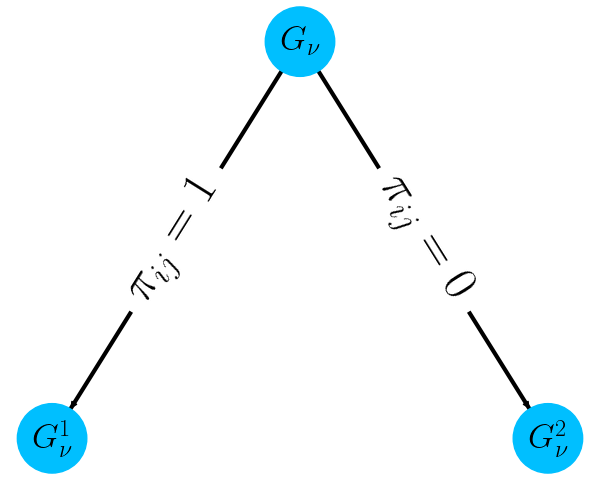
\includegraphics[scale=0.3]{bst_child_nodes.png}}
        \center{\textbf{Ветвление бинарного дерева поиска}}
    \end{minipage}
    \hfill
    
    % \begin{minipage}[b]{1\linewidth}
    %     \fontsize{10pt}{7.2}\selectfont
    %     % \textbf{Алгоритм метода ветвей и границ.}
    %     \bigskip

    %     % Для построения алгоритма МВиГ были разработаны методы исследования вершин дерева на возможность их закрытия.
    %     \bigskip

    %     % В соответствии с техникой МВиГ закрытие вершины в результате исследования, соответствующего ей множества $G_\nu$ возможно \textbf{в трех случаях}:
    % \end{minipage}

\end{frame}

\begin{frame}
    \frametitle{Комбинаторная модель}
    \justifying
    \begin{minipage}[t]{1\linewidth}
        \fontsize{9pt}{7.2}\selectfont

        При формировании дерева ветвлений различаются два типа шагов: <<прямой>> и <<обратный>>. 
    \end{minipage}
    
    \begin{minipage}[b]{0.5\linewidth}
        \fontsize{9pt}{7.2}\selectfont
        \textbf{Прямой шаг} -- это движение «в глубину» по той же ветви дерева, реализующее очередное разбиение множества $G_\nu$ на два потомка.
        \bigskip

        \textbf{Обратный шаг} -- переход к одному из ранее сформированных подмножеств. 
        \bigskip

        Обратный шаг делается в том случае, когда: 
        \begin{itemize}
            \item  получено множество $G_\nu$, состоящее из единственного элемента;
            \item  получено множество $G_\nu$  при наборе значений переменных $\pi_{ij}$ пусто. 
        \end{itemize}
    \end{minipage}
    \hfill
    \begin{minipage}[b]{0.47\linewidth}
        
        \center{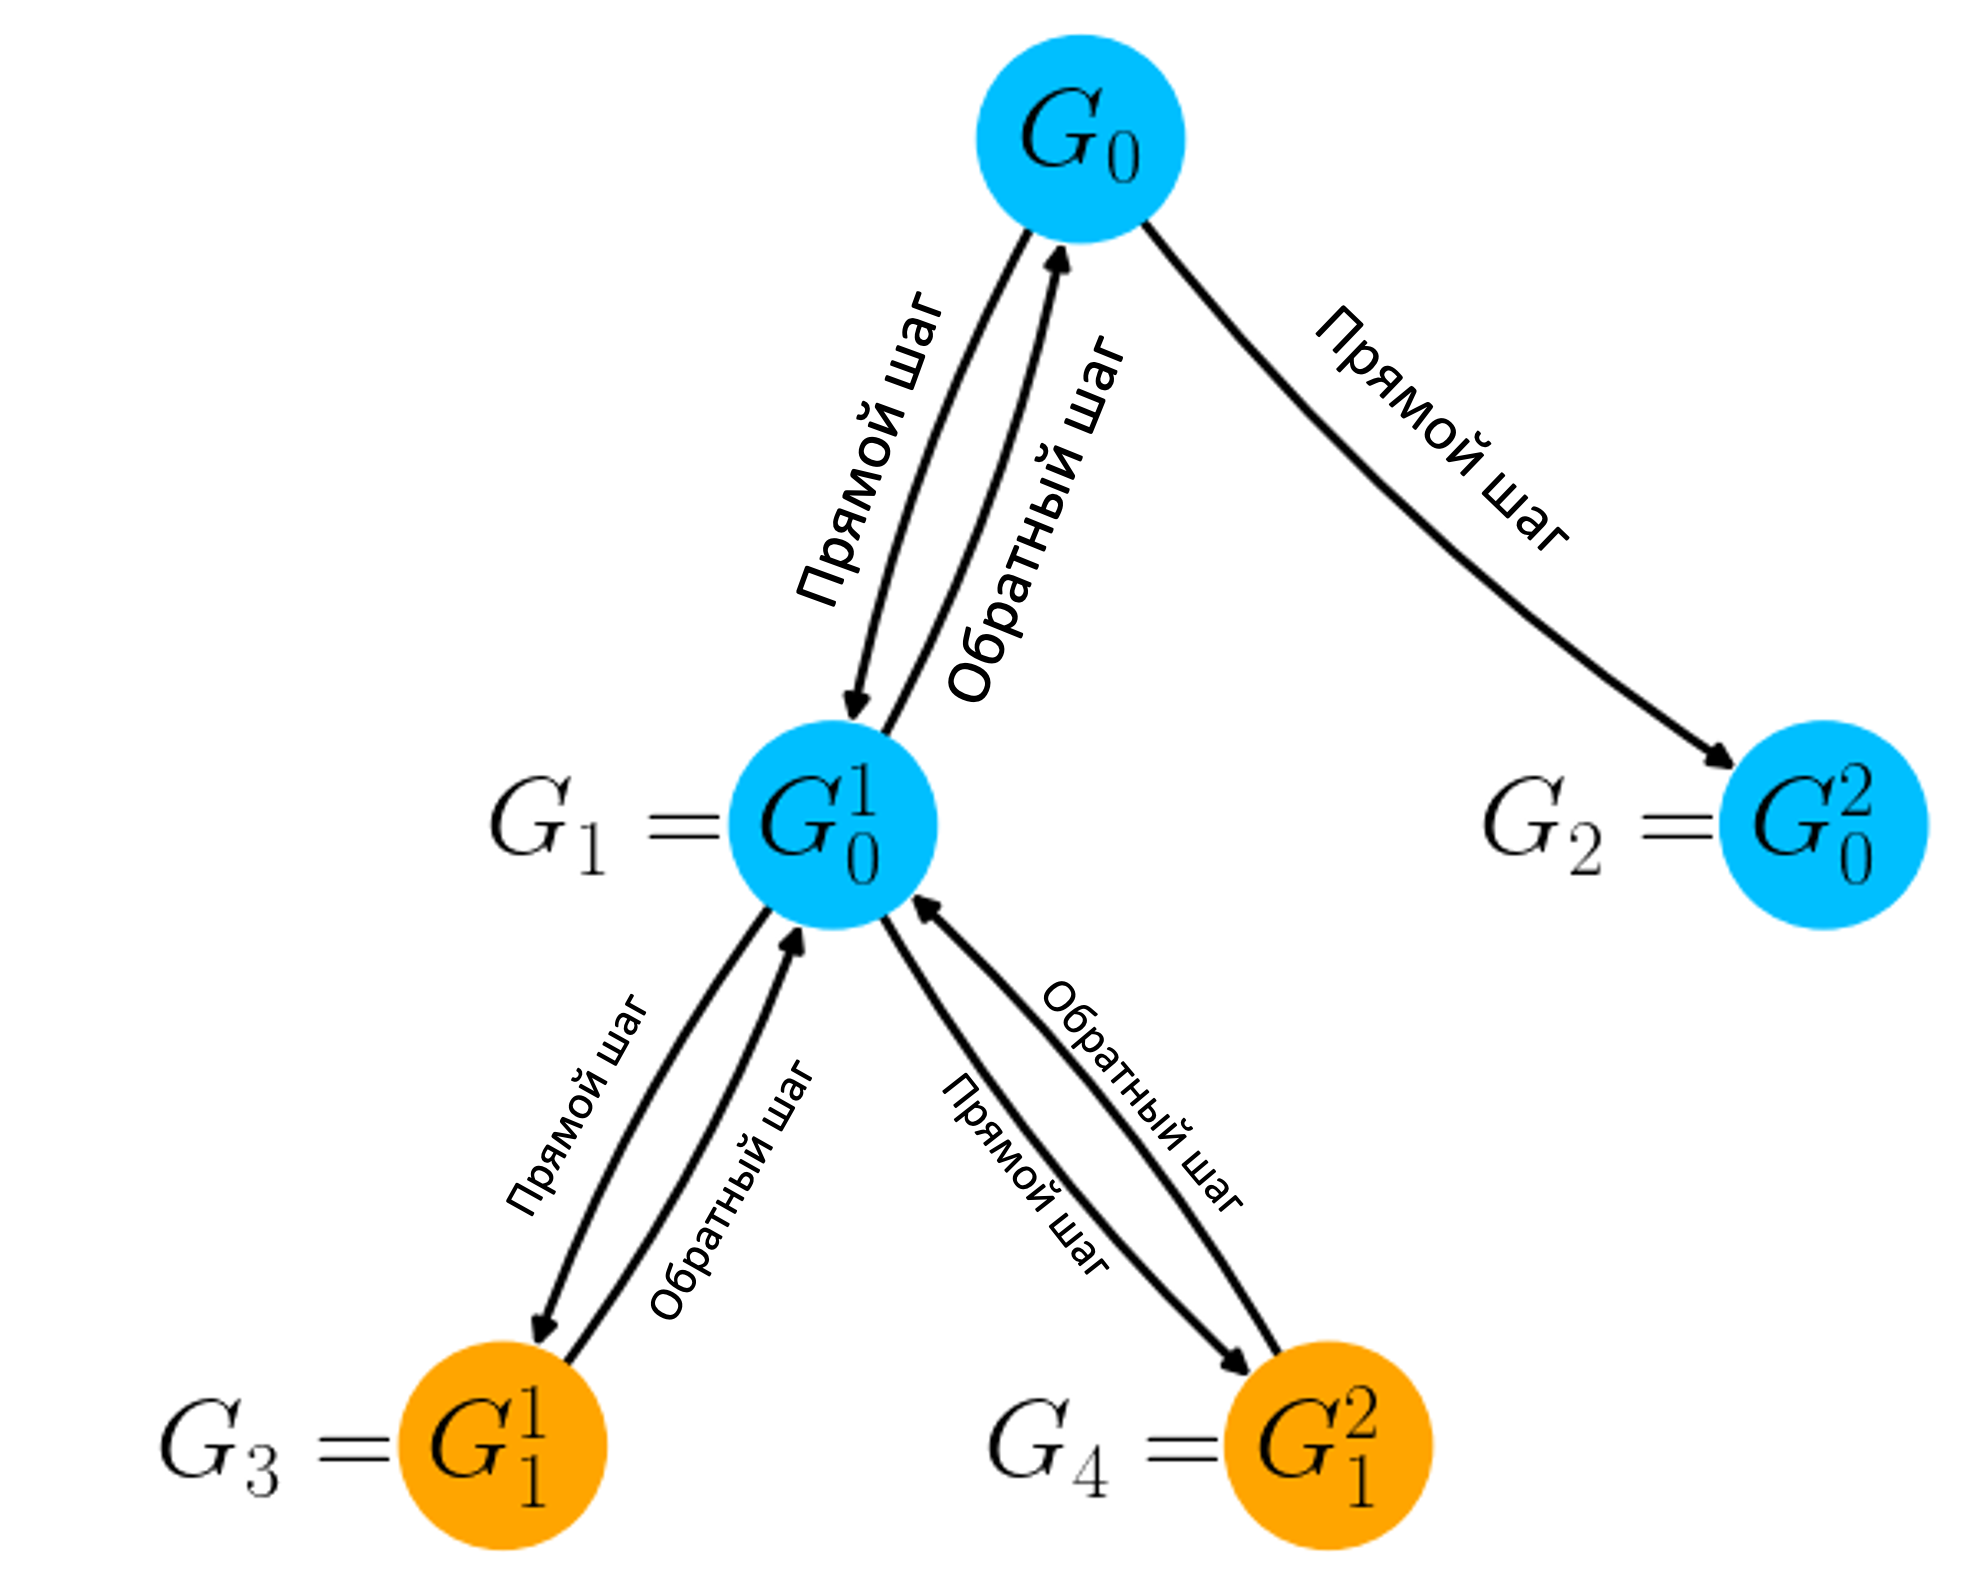
\includegraphics[scale=0.4]{tree_traversal.png}}
        \center{\textbf{Движение по дереву поиска}}
    \end{minipage}
    \hfill


\end{frame}

\begin{frame}
    \frametitle{Алгоритм ветвей и границ}
    \justifying
    В соответствии с техникой МВиГ \textbf{закрытие} вершины в результате исследования множества $G_\nu$ возможно в трех случаях.
    \bigskip

    \underline{\textit{\textbf{Случай 1.}}} Множество $G_\nu$ -- пусто, т.е. доказано, что в множестве $G_\nu$ при данном наборе фиксированных и запрещенных переменных $\pi_{ij}$ нет ни одной допустимой расстановки $P$.
    \bigskip

    \underline{\textit{\textbf{Случай 2.}}} Доказано, что в множестве $G_\nu$ не может быть допустимой расстановки $P$ с меньшим значением целевой функции (19), чем у лучшей расстановки $\widehat{P}$ из уже найденных. 
    \bigskip 
    
    \underline{\textit{\textbf{Случай 3.}}} Найдено оптимальное решение на множестве $G_\nu$.
    % Прежде чем рассмотреть эти три случая, запишем важное свойство любого множеств $G_\nu$, являющееся следствием принятого правила выбора свободной переменной для разбиения очередного множества $G_\nu$ при прямом шаге.

\end{frame}

\begin{frame}
    \frametitle{Алгоритм ветвей и границ}
    \justifying

    \textbf{Случай 1}  состоит в установлении факта невозможности выполнения \textbf{требований 1 -- 3} для текущего множества $G_\nu$,  введенных ранее при определении допустимой расстановки.
    \medskip

    \textbf{Случай 2} и \textbf{Случай 3}. На каждом узле проводится оценка <<недопокрытия>> в виде суммы

    \begin{displaymath}
        W\left(G_\nu\right) = w_1\left(G_\nu \right) + w_2\left(G_\nu \right). 
    \end{displaymath}

    \begin{itemize}
        \item $w_1 \left(G_\nu \right)$ -- сумма все частичных <<недопокрытий>> слева от точки размещения и величины радиуса телекоммуникационного покрытия, размещаемой БС;
        \item $w_2 \left(G_\nu \right)$ вычисляется для <<недопокрытия>> справа на части $\beta$ до конца всего отрезка $L$ (точки $a_{n+1}$).
    \end{itemize}
    Оценку $w_2 \left(G_\nu \right)$ получим релаксацией условий, определяющих допустимую расстановку БС на участке $\beta$. Найдем такое подмножество $S_\beta$ множества $S$, состоящее из еще не размещенных БС и дающее минимальное <<недопокрытие>> на участке $\beta$ при выполнении только стоимостного ограничения. 
    
\end{frame}

\begin{frame}
    
    \frametitle{Алгоритм ветвей и границ}
    \fontsize{8pt}{7.2}\selectfont
    Для этого сформулируем следующую задачу булева программирования.

    \underline{\textit{\textbf{Задача 2.}}}
    \begin{displaymath}\label{present:task2}
        z = |\beta| - \sum\limits_{x_j \in S_\beta} 2 \cdot r_j x_j \rightarrow min.
    \end{displaymath}

    \begin{displaymath}\label{eq:part4_task2_cost}
        \sum\limits_{x_j \in S_\beta} c_j x_j \leqslant C',
    \end{displaymath}

    \begin{displaymath}\label{eq:part4_task2_m}
        \sum\limits_{x_j \in S_\beta} x_j \leqslant m,
    \end{displaymath}

    \begin{displaymath}
        x_j \in \{0, 1\},
    \end{displaymath}
    где $|\beta|$ -- длина отрезка отрезка  $\beta$, $m$ -- число свободных мест для БС на отрезке $\beta$, $c_j$ -- стоимость неразмещенных БС, $C'$ -- бюджет.

    \bigskip
    Эффективность использования оценки в методе ветвей и границ определяется точностью оценки и временем ее вычисления. \underline{\textit{\textbf{Задача 2}}} -- это задача ЦЛП, являющаяся труднорешаемой. При снятии любого одного из ограничений \underline{\textit{\textbf{задача 2}}} представляет собой целочисленную задачу о ранце с эффективным псевдополиномиальным алгоритмом решения. При снятии условия целочисленности переменных $x_j$ \underline{\textit{\textbf{задача 2}}} представляет собой задачу линейного программирования, для решения которой существует эффективный симплекс метод.
 
    \bigskip
    Если множество $G_\nu$ получено из материнского добавлением условия $\pi_{ij}=0$, то оценка $W(G_\nu)$ равна оценке материнского множества.

\end{frame}

\begin{frame}
    \fontsize{8pt}{7.2}\selectfont
    \frametitle{Алгоритм ветвей и границ}
    \justifying
    Если для найденной расстановки $P$ выполняются требования 1 – 3, которые для единственной расстановки легко проверяются, и

    \begin{displaymath}
        f(P) < f(\widehat{P}),
    \end{displaymath}
    то $f(P)$ принимается за новый рекорд $f(\widehat{P})$, расстановка $P$ становиться новым рекордным решением $\widehat{P}$ и выполняется шаг обратного хода по дереву поиска. Если неравенство не выполняется, то рекорд остается прежним и выполняется шаг обратного хода.

    \bigskip
    Работа алгоритма МВиГ заканчивается, когда все вершины дерева поиска закрыты, при этом решение задачи: 

    \begin{displaymath}
        P^{*} = \widehat{P},  f(P^*) = f(\widehat{P}).
    \end{displaymath}

    \bigskip
    \bigskip
    % Обе задачи, в виде ЦЛП и в виде комбинаторной модели в экстремальной форме относятся к широкому к \textbf{классу задач размещения мощностей}. Отличительной особенностью рассмотренных задач является наличие условия на связь между размещаемыми объектами и линейная контролируемая территория.
\end{frame}

\begin{frame}
    \frametitle{Численный результат}

    Требуется разместить весь набор $m$ имеющихся однотипных БС. Множество всех возможных вариантов комбинаций $m$ БС на  $n$ местах запишем как $\Gamma$. Общее количество $\gamma \in \Gamma$:
   
    \begin{displaymath}
    \gamma = C_n^m \times m!.
    \end{displaymath} 

    В МВиГ отпустим ограничение на межконцевую задержку.
    
    \bigskip

    Характеристика сравнения двух моделей --  \textbf{количество}  \textbf{пройденных}  \textbf{узлов} в ходе поиска оптимального значения.
    
    \bigskip
    В таблице показаны результаты решения задач для различного числа количества размещения и количества станций с использованием полного перебора (МПП), МВиГ и ЦЛП. Для каждого набора станций и набора размещений были рассчитаны 10 примеров с различными числовыми входными данными. 

    % Как видно из результов, представленных в таблице, при увеличении размерностей задачи, алгоритм МВиГ позволяет найти решение быстрее в ходе движения по дереву поиска.

    % \begin{table}[b]\centering
    %     \caption{Результаты численного решения.}\label{tab:problems_BF_BnB_ILP}
    %     \begin{tabular}{|l|l|l|l|l|}
    %     \hline
    %     \textbf{Места} & \textbf{Станции} &	\textbf{Полный}& \textbf{МВиГ} & \textbf{ЦЛП} \\ 
    %     \textbf{размещения} &  &	\textbf{перебор}&  &  \\
    %     \hline
    %     7 &		5 &	17550  &	933 &		\textbf{753}\\
    %     9 &		5 &	71090  &	6478 &		\textbf{2669}\\
    %     10 &	5 &	126180 &	\textbf{1041} &		8551\\
    %     12 &	6 &	-- &		\textbf{8294} &		38569\\
    %     13 & 	6 &	-- &		\textbf{18485} &	30369\\
    %     \hline
    %     \end{tabular}
    % \end{table}

\end{frame}

\begin{frame}
    % \frametitle{Численный результат}
    % \fontsize{12pt}{7.2}\selectfont
    \small
    \begin{table}
        \caption{Результаты численного решения}\label{tab:models_comparation}
        \begin{tabular}{|ccc|*{3}{c}|} \cline{3-6}
        \hline
        \textbf{Число мест} & \textbf{Число} &\textbf{Количество} & \multicolumn{3}{c|}{\textbf{Количество пройденных}}\\ 
        \textbf{размещения,} & \textbf{БС,} & \textbf{вариантов} & \multicolumn{3}{c|}{\textbf{узлов дерева поиска, $\nu$}}\\
        \cline{4-6}
        \textbf{$n$} & \textbf{$m$} &\textbf{размещения, $\gamma$} & \textbf{МПП}& \textbf{МВиГ} & \textbf{ЦЛП} \\ 
        \hline
        7 &  4 & 840 & 3122 & 360 &  \textbf{275} \\
        7 &  5 & 2 520 & 16 114 & 560  &  \textbf{45}  \\
        7 &  6 & 5 040 & 59 564 & 364  &  \textbf{19}  \\
        8 &  4 & 1 680 &  4954 &  434 &   \textbf{189} \\
        8 &  5 & 6 720 & 6720 & \textbf{852}  &  878 \\
        8 &  6 & 20 160 &  15 9170 & 592  & \textbf{185}  \\
        9  &  4 & 3 024 & 9 882 & \textbf{458} & 5511 \\
        9  &  5 & 15 120&  58 190 &  \textbf{768} &  1236\\
        9  &  6 & 60 480&  366 512 &  \textbf{720} & 13294 \\
        10 &  4 & 5 040&  14 868&  \textbf{800}&  6243\\
        10 &	5 & 30 240&  113 932&  \textbf{414}&  8043\\
        10 &	6 & 151 200&  828 952&  \textbf{40 872}&  71587\\
        11 &  4 & 7 920& 23 482&  \textbf{354} & 15538\\
        11 &	5 & 55 440& 204 894& \textbf{9 138}&  74440\\
        11 &	6 & 332 640& 1 592 500 & \textbf{88 002} & 413 767 \\
        \hline
        \end{tabular}
      \end{table} 
\end{frame}

\begin{frame}
    \frametitle{Последовательность лучших решений}
    \fontsize{8pt}{7.2}\selectfont
    Рассмотрим \textbf{задачу 1.}

    \begin{displaymath}
        f(P^*) = min \{f(P), P \in G \}.
    \end{displaymath}

    Построим для этой задачи последовательность $\Gamma' = P^1, P^2, ... ,P^k$ допустимых расстановок (решений) множества $G$ для заданного $k$, где 
    \begin{align}
        f(P^1) &= f(P^*), \nonumber  \\
        f(P^2) &= extr\{ f(P), P \in G \textbackslash P^1 \}, \nonumber \\
        ... \nonumber \\
        f(P^k) &= extr\{ f(P), P \in G \textbackslash P^1 \cup P^2 \cup ... P^k \}.
    \end{align} 
    
    Для итерационной процедура нахождения последовательности лучших решений достаточно строгое неравенство $f(P) < f(\widehat{P})$ в алгоритме МВиГ заменить следующим нестрогим неравенством 

    \begin{align}
        \label{eq:part4_is_less_than_record_d}
        f(P) \leqslant f(\widehat{P}) + d,
    \end{align}
    где $d = \varepsilon \cdot L > 0, \varepsilon$ -- заданное отклонение в процентах, и запоминать все рекорды, полученные в процессе решения задачи.

\end{frame}

% \begin{frame}
%     \frametitle{Задача с линейной топологией}
%     \fontsize{8pt}{7.2}\selectfont
%     % \justifying
%     \begin{itemize}
%         \item Математическая модель задачи ЦЛП (1) - (18) написана и решена в Matlab Optimization Toolbox.
%     \end{itemize}

%     \begin{minipage}[c]{0.4\linewidth}
%         \fontsize{8pt}{7.2}\selectfont
%         \bigskip
%         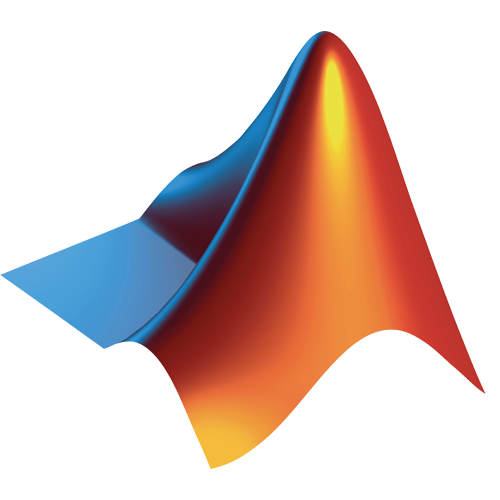
\includegraphics[scale=0.09]{matlab.png}

%     \end{minipage}
%     \textit{https://github.com/m0000Amir/ILP}
%     \bigskip
%     \bigskip
    
%     \begin{itemize}
%         \item Математическая модель комбинаторной задачи и алгоритм МВиГ написаны на языке Python. Задача ЦЛП оценки недопокрытия справа решалась в Gurobi Optimization.
%     \end{itemize}

%     % \begin{minipage}[c]{0.45\linewidth}
%     %     \fontsize{8pt}{7.2}\selectfont
%     %     \bigskip
%     %     
\includegraphics[scale=0.1]{python.png}

%     % \end{minipage}

%     % \begin{minipage}[c]{0.45\linewidth}
%     %     \fontsize{8pt}{7.2}\selectfont
%     %     \bigskip
%     %     
\includegraphics[scale=0.26]{gurobi.png}

%     % \end{minipage}

%     \begin{minipage}[c]{0.45\linewidth}
%         \fontsize{8pt}{7.2}\selectfont
%         \bigskip
%         
\includegraphics[scale=0.1]{python.png}
        
%     \end{minipage}
%     % \hfill
%     % \vrule{}
%     % \hfill  
%     \begin{minipage}[c]{0.45\linewidth}
%         
\includegraphics[scale=0.26]{gurobi.png}

%     \end{minipage}

%     \bigskip
%     \textit{https://github.com/m0000Amir/BST\_BS\_types\_set}


%     % \begin{minipage}[c]{0.47\linewidth}
%     %     \center{
\includegraphics[scale=0.2]{gurobi.png}}
%     %     \center{\textbf{Вершины $A$.}}
%     % \end{minipage}
    
% \end{frame}

\begin{frame}
    \frametitle{Программный комплекс}
    \fontsize{8pt}{7.2}\selectfont
    % \justifying
    \begin{itemize}
        \item Математическая модель ЦЛП (1) - (16) написана и решена в Matlab Optimization Toolbox. \textit{https://github.com/m0000Amir/ILP}
        \item Для комбинаторной модели разработан программный комплекс. \textit{https://github.com/m0000Amir/BST\_BS\_types\_set}
    \end{itemize}
    % Математическая модель задачи ЦЛП (1) - (18) написана и решена в Matlab Optimization Toolbox. \textit{https://github.com/m0000Amir/ILP}
    
    % \bigskip
    % Для комбинаторной модели разработан программный комплекс. \textit{https://github.com/m0000Amir/BST\_BS\_types\_set}



    \begin{minipage}[b]{0.5\linewidth}
        \fontsize{9pt}{7.2}\selectfont
        \center{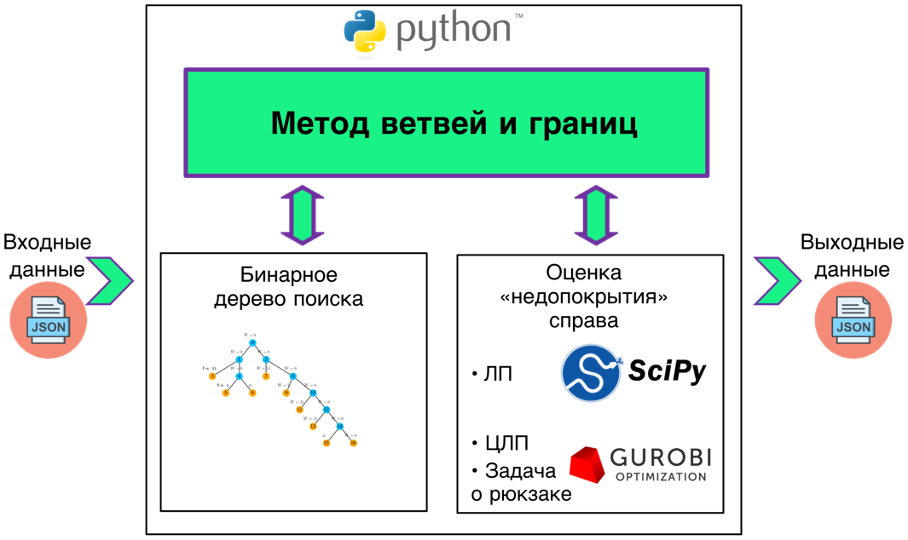
\includegraphics[scale=0.2]{program_computer.png}}
        \center{\textbf{Структура программного комплекса}}
    \end{minipage}
    \hfill
    \begin{minipage}[b]{0.45\linewidth}
        
        \center{
\includegraphics[scale=0.1]{program_mukhtarov.jpeg}}
        \center{\textbf{Свидетельство о государственной регистрации программы для ЭВМ}}
    \end{minipage}
    \bigskip



    
\end{frame}

\begin{frame}
    \frametitle{Выводы по Положениям 1, 2 и 3}
    \fontsize{8pt}{7.2}\selectfont

    \textbf{Представлены:}
    \begin{itemize}
        \item математическая модель ЦЛП;
        \item комбинаторная модель в экстремальной форме;
        \item специальный алгоритм МВиГ для комбинаторной модели;
        \item итерационная процедура нахождения последовательности лучших решений.
    \end{itemize}

    \bigskip
    \textbf{Основные публикации:}
    \begin{minipage}[c]{1\linewidth}
        \fontsize{4pt}{5.2}\selectfont
        \begin{enumerate}
            \item \textit{Иванов, Р. Е. Задача оптимального размещения заданного множества базовых станций беспроводной сети связи с линейной топологией [Текст] / Р. Е. Иванов, А. А. Мухтаров, О. Ю. Першин // Автоматизация, телемеханизация и связь в нефтяной промышленности. — 2019. — Т. 549, No 4. — С. 39—45.};
            
            \item \textit{Ivanov,R.A Problem of Optimal Location of Given Set of Base Sta­tions in Wireless Networks with Linear Topology[Текст]/ R. Ivanov,A. Mukhtarov, O. Pershin // Communications in Computer and Infor­mation Science. –– 2019. –– Vol. 1141 CCIS. –– P. 53––64. –– (Scopus,WoS)};
            
            \item \textit{On Optimal Placement of Base Stations in Wireless Broadband Net­works to Control a Linear Section with End-to-End Delay Limited[Текст]/ A. Mukhtarov [et al.] // Communications in Computer andInformation Science. –– 2020. –– Vol. 1337. –– P. 30––42};
            
            \item \textit{Вишневский, В. М. Расчёт характеристик тандемной сети с фиксированными длинами входящих пакетов методом машинного обучения [Текст] / В. М. Вишневский, А. А. Ларионов, А. А. Мухтаров // Материалы 13-й конференции с международным участием "Новые информационные технологии в исследовании сложных структур"(ICAM 2020, Томск). — 2020. — С. 82.};
            \item \textit{Mukhtarov A. A., Sokolov A. M. A base station placement of an wireless network with linear topology and a network performance evaluation with NS-3 // Информационно-телекоммуникационные технологии и математическое моделирование высокотехнологичных систем: материалы Всероссийской конференции с международным участием, Москва, 19–23 апреля 2021 года, 2021. С. 425–430;}
            \item \textit{Лазарева,В. Е.Расчёт межконцевых задержек и длин очередей в многошаговой тандемной сети с применением методов машинного обучения [текст] / В. Е. Лазарева, А. А. Ларионов, А. А. Мухтаров //Материалы Всероссийской конференции с международным уча­стием "Информационно-телекоммуникационные технологии и мате­матическое моделирование высокотехнологичных систем"(Москва,2020). — 2020. — с. 43—48.20.}
            \item \textit{Larionov, A. A. The calibration method of a tandem queueing model with PH service time using NS-3 simulation of a multihop wireless network [Текст] / A. A. Larionov, A. A. Mukhtarov, A. M. Sokolov // Journal of Physics: Conference Series. –– 2021. –– Vol. 2091, no. 1. –– P. 012030}.
            \item \textit{Оптимальное размещения базовых станций в рамках комплексного проектирования беспроводной сети [Текст] / О. Ю. Першин, В. М. Вишневский, А. А. Мухтаров, А. А. Ларионов // Информационные технологии и вычислительные системы. — 2022. — No 1. — С. 12—25.}
        \end{enumerate}
    \end{minipage}

\end{frame}

% \section{Положение 4}
\begin{frame}
    \begin{center}
        {\textbf{Положение 4} - Математические модели для задач проектирования БШС с ячеистой топологией для обслуживания множества рассредоточенных объектов.}
    \end{center}

    \center{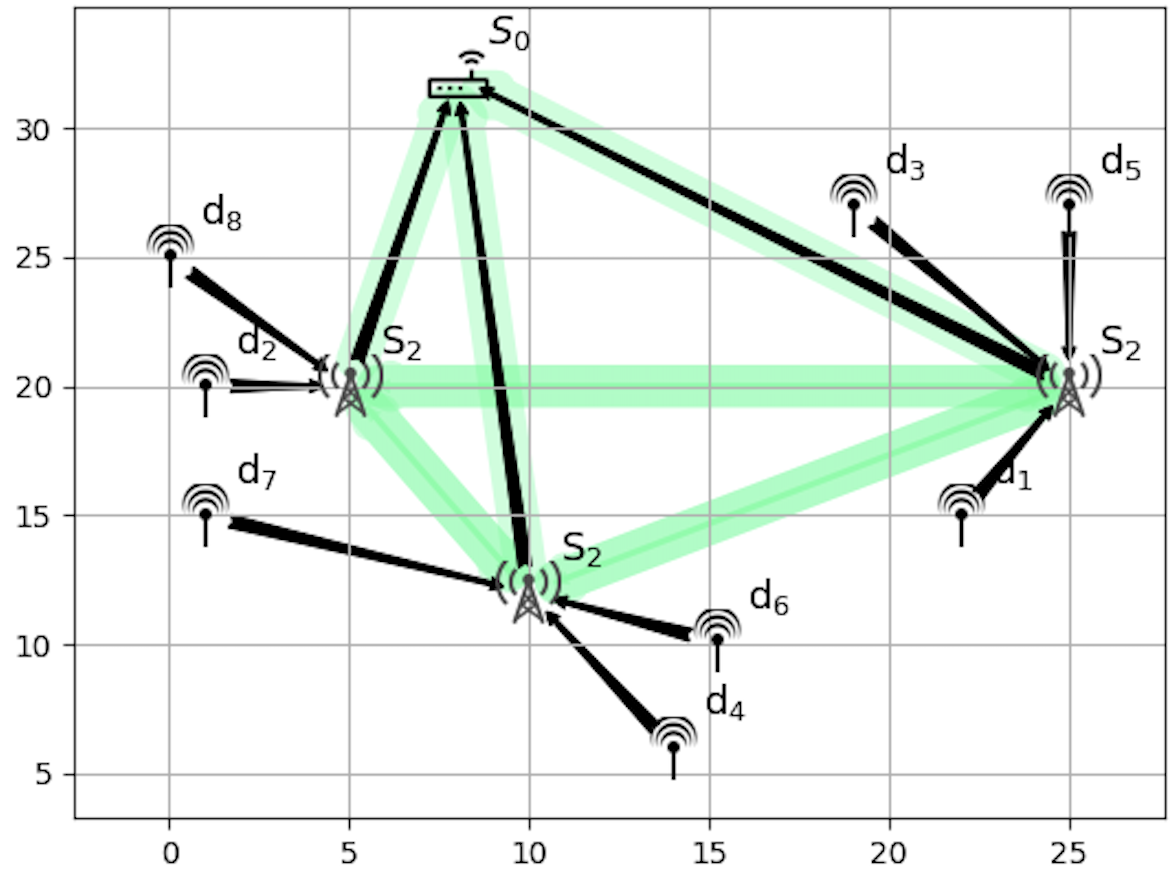
\includegraphics[scale=0.25]{presentation_part_4.png}}
    \fontsize{8pt}{7.2}\selectfont
        \center{\textbf{БШС с ячеистой топологией для обслуживания множества рассредоточенных объектов}}

\end{frame}



\begin{frame}
    \frametitle{Постановка задачи}
    \fontsize{8pt}{7.2}\selectfont
    \justifying
    Задано множество вершин $A = a_i$, $i=\overline{0,n}$. Каждая вершина $a_i$ имеет координаты $\left\{ x_i, y_i \right\}$.
    
    \begin{minipage}[b]{0.5\linewidth}
        \bigskip

        Множество $A$ состоит из двух подмножеств: 
        \begin{itemize}
        \item $A_1$ -- множество вершин, с которых необходимо собирать информацию. Каждой вершине $a_i$ приписана   величина $\vartheta_i$ -- максимальный объем информации, снимаемой с объекта;
        \item $A_2$ -- множество возможных мест размещения БС. 
        \end{itemize}

        По определению

        $$
        A_1 \cup A_2 = A;
        $$

        $$
        A_1 \cap A_2 = \varnothing.
        $$   

    \end{minipage}     
    \hfill
    \begin{minipage}[b]{0.5\linewidth}
        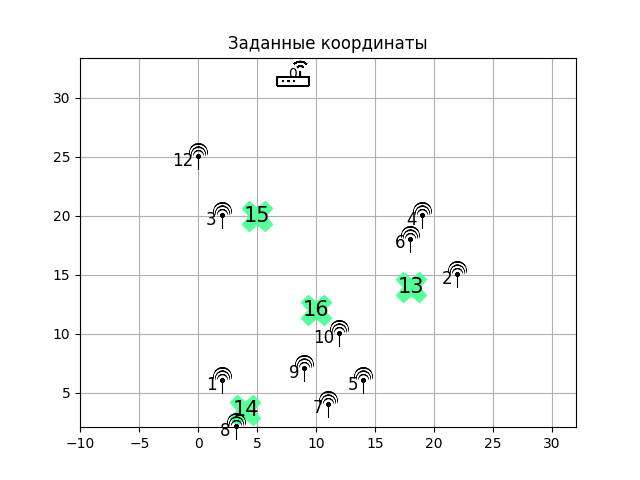
\includegraphics[scale=0.3]{bsp_input_data.png}
        \center{\textbf{Вершины $A$.}}
    \end{minipage}
    \medskip

    $
    A_1 = \left\{a_i \right\}, i= \overline{1,n_1};
    $ и $
    A_2 = \left\{ a_i  \right\}, i= \overline{n_1+1,n}.
    $

    \textbf{Предложены}:
    \begin{itemize}
        \item \textbf{модель линейного программирования (ЛП) нахождения допустимого потока информации при заданных местах размещения БС;}
        \item \textbf{модель частично целочисленного программирования (ЧЦЛП) минимизации суммарной стоимости размещения  БС.}
    \end{itemize}

\end{frame}


\begin{frame}
    \frametitle{Задача поиска допустимого потока информации}
    \fontsize{10pt}{7.2}\selectfont
    \justifying

    \bigskip


    Множество $A_2$ будем идентифицировать не только как место размещения, но и как размещенная БС на ней.
    
    \bigskip
    
    Каждой вершине из $A_2$ приписаны три параметра $s_i = \left\{ r_i, \{R_{ij}\},\vartheta_i \right\}$, где $r_i$ -- максимальный радиус телекоммуникационного покрытия БС; $R_{ij}$ -- максимальный радиус телекоммуникационной связи между $i$-ой и $j$-ой БС и $\vartheta_i$ -- максимальный объем получаемый информации в единицу времени. 
    
    \bigskip
    
    Задана шлюз $s_0 = \left\{ r_0, R_0, \vartheta_0 \right\} $ с координатами $\left\{x_0, y_0 \right\}$. Задано условие, что со шлюзом и между собой могут быть связаны только вершины множества $A_2$.

\end{frame}


\begin{frame}
    \frametitle{Задача поиска допустимого потока информации}

    \textbf{Требуется} проверить, что при заданных наборе и размещении БС вся имеющаяся информация с объектов (множество $A_1$) может быть собрана и передана системой БС (множество $A_2$) до шлюза $s_0$.

    \bigskip

    Составим граф $ H = \left\{A,E \right\} $ для возможного потока информации между вершинами множества $ A = A_1 \cup A_2 $. 
    
    \medskip
    Матрица смежности $E = \left\{ e_{ij} \right\}$ графа $H$ строится по следующим правилам:

% \begin{itemize}
%     \item $e_{ij} = 1$, если расстояние между $i$-ым объектом ($a_i \in A_1$) и $j$-ым местом размещения станции ($a_j \in A_2$) не более радиуса покрытия для станции соответствующего этой вершине типа; 
%     \item $e_{ij} = 1$, если расстояние между $i$-ым местом размещения ($a_i \in A_2$) и $j$-ым местом размещения  ($a_j \in A_2$), не более радиуса связи той станции, у которой радиус связи не больше радиуса связи другой станции;
%     \item $e_{i0} = 1$, если расстояние от вершины $a_i \in A_2$ до шлюза не более $R_{i0}$;
%     \item $e_{ij} = 0$, во всех остальных случаях.
% \end{itemize}

    \bigskip

    \begin{minipage}[c]{0.47\linewidth}
        % \fontsize{10pt}{7.2}\selectfont
        $$
        e_{ij} = 
        \begin{cases}
        1& \text{, если $ ||a_i - a_j|| \leqslant r_j, \forall a_i \in A_1, a_j \in A_2$;} \\
        1 & \text{, если $ ||a_i - a_j|| \leqslant R_{ij}, \forall a_i \in A_2, a_j \in A_2, a_i \neq a_j$;} \\
        1 & \text{, если $ ||a_i - a_0|| \leqslant R_{i0}, \forall a_j \in A_2$;} \\
        0 & \text{, во всех остальных случаях.}
        \end{cases}
        $$
    \end{minipage}


\end{frame}



\begin{frame}
    \frametitle{Задача поиска допустимого потока информации}
    \fontsize{10pt}{5.2}\selectfont
    \justifying

    % С помощью полученной матрицы смежности $E$, необходимо подготовить условия ограничения для величины потока в каналах.

    Введем переменные $x_{ij} \geqslant 0$, определяющее количество информации, передаваемой в единицу времени по дуге $e_{ij}$ графа $H$.

    Каждый объект множества $A_1$ генерирует пакеты объемом $\vartheta_i$ в единицу времени. Для ребра $e_{ij}, i = \overline{1,n_1}, j = \overline{n_1+1,n}$ величина потока равна весу $\vartheta_i$:

    \begin{equation}\label{eq:part2_1.1}
        \sum_{a_j \in \Gamma^+(a_i)} x_{ij} = \vartheta_i, \forall a_i, i=\overline{1, n_1},
    \end{equation}
    где $\Gamma^+(a_i)$ – множество вершин на графе $H$, в которые входят дуги, исходящие из вершины $a_i$. 

    % Для каждой вершины $a_i,  a_i \in A_2$ необходимо обеспечить выполнения условия баланса между потоком входящем в эту вершину от объектов множества $A_1$, а также других БС множества $A_2$ и выходящего потока из данной вершины. 

    Сумма входящих и выходящих потоков для любой вершины $a_i$  множества $A_2$ должна быть равна нулю:

    \begin{equation}\label{eq:part2_1.2}
        \sum_{a_j \in \Gamma_1^-(a_i)} x_{ji} + \sum_{a_j \in \Gamma_2^-(a_i)} x_{ji} -  \sum_{a_j \in \Gamma_2^+(a_i)} x_{ij} =0 ,\forall a_i \in A_2. 
    \end{equation}

    Здесь множество $\Gamma_1^-(a_i)$ -- вершины множества $A_1$, из которых выходят дуги, входящие в вершину $a_i$; $\Gamma_2^-(a_i)$ –- вершины множества $A_2$, из которых выходят дуги, входящие в  вершину $a_i$; $\Gamma_2^+(a_i)$ –- вершины множества $A_2$, в которые входят дуги, исходящие из вершины $a_i$.
   

\end{frame}


\begin{frame}

    \fontsize{10pt}{5.2}\selectfont
    \justifying

    Необходимо чтобы на выходе сети собирался весь трафик. Через систему БС на вершинах $a_j, a_j \in A_2$, вся информация от объектов на вершинах $a_i, a_i \in A_1$ поступала  на шлюз $s_0$:

    \begin{equation}\label{eq:part2_1.3}
        \sum_{a_j \in \Gamma_2^-(a_0)} x_{j0} =  \sum_{a_i \in A_1} \vartheta_i;
    \end{equation}


    Поток объема информации в каналах ограничен сверху. В случае каналов передачи от объектов на вершинах $A_1$ до БС на вершинах $A_2$ поток ограничен объемом сгенерированного трафика на объекте $\vartheta_i$:


    \begin{equation}\label{eq:part2_1.4_1}
        x_{ij} \leqslant \vartheta_i, \forall a_i \in A_1, a_j \in A_2.
    \end{equation}

    Объем информации входящий на БС на вершине $a_j, a_j \in A_2$ ограничен пропускной способностью $\vartheta_j$ БС: 


    \begin{equation}\label{eq:part2_1.4_2}
        \sum_{a_i \in \Gamma^-(a_j)} x_{ij} \leqslant \vartheta_j, \forall a_j \in A_2.
    \end{equation}


    Если к системе уравнений ограничений (20) -- (24) добавить целевую функцию

    \begin{equation}
        \label{eq:part2_1.5}
        \sum_{(a_i, a_j) \in A} c_{ij} x_{ij} \rightarrow \min ,
    \end{equation}
    где $c_{ij}$ -- стоимость потока (равна 1, если существует ребро $e_{ij}$). 
    \medskip
    Данная модель является задачей ЛП \textbf{о потоке минимальной стоимости}. 

\end{frame}

\begin{frame}
    \frametitle{Задача поиска допустимого потока информации}
    \fontsize{7pt}{5.2}\selectfont
    \justifying
    \begin{table}[h!]\centering
            
        \begin{tabular}{|c|| c| c c c c c| c c c|}\hline
            
            & $a_0$& $a_1$& $a_2$& $a_3$& $a_4$& $a_5$& $a_6$& $a_7$ & $a_8$\\
            \hline
            \hline
            $a_0$ & 0&	0&	0&	0&	0&	0&	0 &	0&	0\\
            \hline
            $a_1$ & 0&	0&	0&	0&	0&	0&	1 &	0&	0\\
            $a_2$ & 0&	0&	0&	0&	0&	0&	0 &	1&	1\\
            $a_3$ & 0&	0&	0&	0&	0&	0&	1 &	0&	1\\
            $a_4$ & 0&	0&	0&	0&	0&	0&	0 &	1&	1\\
            $a_5$ & 0&	0&	0&	0&	0&	0&	0 &	0&	1\\
            \hline
            $a_6$ & 0&	0&	0&	0&	0&	0&	0 &	0&	1\\
            $a_7$ & 1&	0&	0&	0&	0&	0&	0 &	0&	1\\
            $a_8$ & 1&	0&	0&	0&	0&	0&	1 &	1&	0\\
            \hline
        \end{tabular}\caption{Матрица смежности графа потока $H$}\label{tab:part3_lp_adj_mat}
    \end{table}
    % \end{minipage}
    % \hfill
    % \begin{minipage}[b]{0.6\linewidth}
        
    %     % \begin{figure}[h!]
    %         \centering
    %             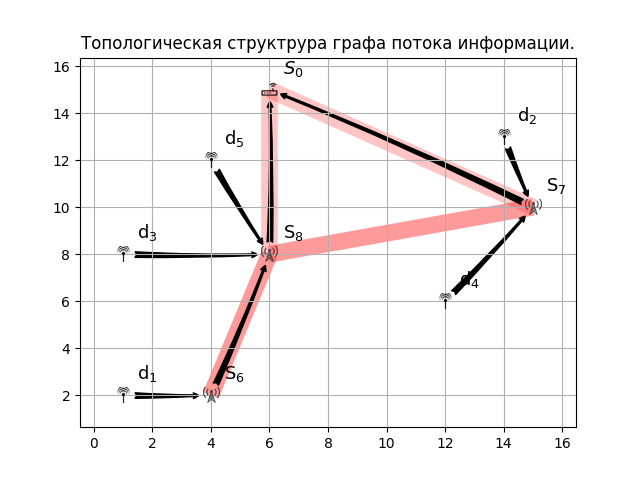
\includegraphics[width=.8\textwidth]{lp_solution.png}
    %         % \caption{Допустимое решение}
    %     % \end{figure}
    %
    \begin{minipage}[b]{0.5\linewidth}
        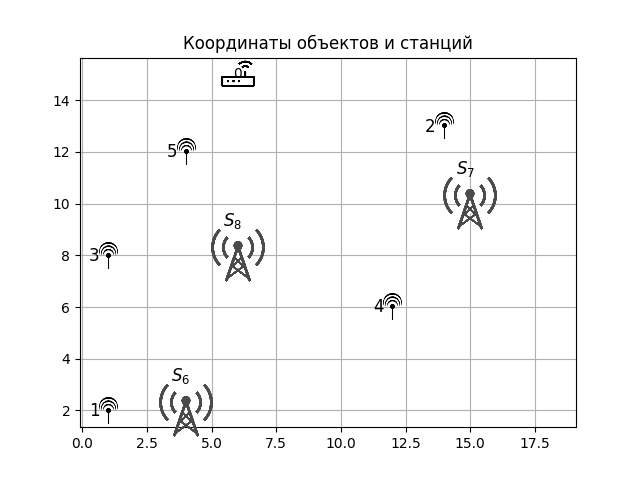
\includegraphics[width=.8\textwidth]{lp_input.png}
        \center{\textbf{Размещение БС}}


    \end{minipage}     
    \hfill
    \begin{minipage}[b]{0.5\linewidth}
        \centering
        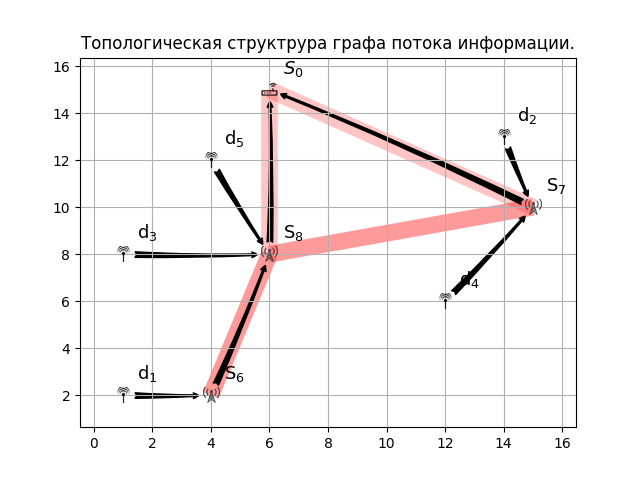
\includegraphics[width=.8\textwidth]{lp_solution.png}
        \center{\textbf{Допустимое решение}}
    \end{minipage}

    На рисунке представлен полученный граф допустимого потока. Красным цветом представлена телекоммуникационная связь между объектами и БС. 

    Стрелками указан полученный граф потока информации от объектов до шлюза. 
\end{frame}

\begin{frame}
    \frametitle{Оптимальное размещение БС на плоскости}
    \justifying

    % Оптимизационная задача размещения типов БС БШС для обеспечения телекоммуникационного покрытия рассредоточенных объектов. 
    Задача имеет ту же постановку как в модели ЛП, теперь  только множество вершин $A_2$ задаются свободными. 

    \bigskip
    
    Задано множество \textbf{типов базовых станций} $S = \{s_j\}$, $j=\overline{1,m}$. Каждой станции приписаны параметры $s_j = \left\{r_j, \{R_{ij}\}, \vartheta_j, c_j \right\}$, где:
    $r_j$ -- максимальный радиус телекоммуникационного покрытия; $R_{ij}$ -- максимальный радиус телекоммуникационной связи между $i$-ой и $j$-ой станциями; $\vartheta_j$ -- максимальный получаемый объем информации в единицу времени; $c_j$ -- стоимость станции.
    
    \bigskip
    % Задана БС специального вида (шлюз) $s_0 = \left\{ \{R_{0j}\}, \vartheta_0 \right\}$ с координатами $\left\{x_0, y_0 \right\}$.  Полагается, что шлюз не имеет соединения напрямую с объектами. 
    % \bigskip
    \textbf{Требуется} разместить базовые станции таким образом, чтобы минимизировать их суммарную стоимость и обеспечить сбор информации со всех рассредоточенных объектов.

\end{frame}

\begin{frame}
    \frametitle{Оптимальное размещение БС на плоскости}
    \fontsize{10pt}{7.2}\selectfont
    % Вместо каждой вершины множества $A_2$ введем $m$ вершин с координатами вершины $a_i$, и различными параметрами станций (множества $D_i$). Полученное множество по всем вершинам назовем $A_2D$.
    % \bigskip

    % Составим граф $H=\left\{AD,E\right\}$, передачи потока информации между вершинами расширенного множествa $AD=A_1 \cup A_2D$ и шлюзом.


    Вместо каждой вершины множества $A_2$ введем $m$ вершин с координатами вершины $a_i$, и различными параметрами станций (множества $D_i$). Полученное множество по новым вершинам назовем $A_2D$. Множество всех вершин теперь$AD=A_1 \cup A_2D$

    \bigskip

    

    Матрица смежности $E = \{e_{ij}\}$ графа $H=\left\{AD,E\right\}$ строится по следующим правилам.
    
    \begin{minipage}[c]{0.47\linewidth}
        \fontsize{10pt}{7.2}\selectfont
        $$
        e_{ij} = 
        \begin{cases}
        1& \text{, если $ ||a_i - a_j|| \leqslant r_j, \forall a_i \in A_1, a_j \in A_2D$;} \\
        1 & \text{, если $ ||a_i - a_j|| \leqslant R_{ij}, \forall a_i \in D_i, a_j \in D_j$;} \\
        1 & \text{, если $ ||a_i - a_0|| \leqslant R_{i0}, \forall a_i \in A_2D$;} \\
        0 & \text{, во всех остальных случаях.}
        \end{cases}
        $$
        \bigskip

    \end{minipage}

    С помощью полученного графа потока опишем ограничения для задачи ЧЦЛП.
        
\end{frame}

\begin{frame}
    \frametitle{Оптимальное размещение БС на плоскости}
    \fontsize{8pt}{7.2}\selectfont

    

    Введем булевы переменные $z_{ij} = \{0, 1\}$, $ i = \overline{1,n_1}, j = \overline{n_1+1, \ n \cdot m}$, определяющие наличие соединения между объектом в точке $a_i, a_i \in A_1$  и БС, размещенной в точке $a_j, a_j \in A_2D$.


    Все объекты, размещенные на вершинах $A_1$, могут одновременно поддерживать соединение только с одной БС:


    \begin{equation}\label{eq:part3_only_1_link_from_device}
        \sum_{a_j \in \Gamma_2^+(a_i)} z_{ij} = 1, \forall a_i, i =\overline{1, n_1},
    \end{equation} 
    где $\Gamma^+(a_i)$ -- множество вершин на графе $H$, в которые входят дуги, исходящие из вершины $a_i$.

    \bigskip

    Введем потоковые переменные $x_{ij} \in \mathbb{R}^+$, определяющие количество информации, передаваемой в единицу времени по дуге $e_{ij}$ графа $H$. Необходимо, чтобы сумма входящих и выходящих потоков для любой $j$-ой вершины множества $A_2D$ была равна нулю  

    \begin{equation}\label{eq:part3_sta_io_flows} 
        \sum_{a_i \in \Gamma_1^-(a_j)} z_{ij} \cdot \vartheta_i + \sum_{a_i \in \Gamma_2^-(a_j)} x_{ij} -  \sum_{a_i \in \Gamma_2^+(a_j)} x_{ji} =0 ,\forall a_j \in A_2. 
    \end{equation} 

    Здесь множество $\Gamma_1^-(a_i)$ -- вершины множества $A_1$, из которых выходят дуги, входящие в вершину $a_i$; $\Gamma_2^-(a_i)$ -- вершины множества $A_2D$, из которых выходят дуги, входящие в  вершину $a_i$; $\Gamma_2^+(a_i)$ -- вершины множества $A_2D$, в которые входят дуги, исходящие из вершины  $a_i$.



\end{frame}

\begin{frame}
    \frametitle{Оптимальное размещение БС на плоскости}
    \fontsize{8pt}{7.2}\selectfont

    Через систему БС вся информация от объектов  должна поступить на шлюз $s_0$ 
    \begin{equation}\label{eq:part3_device2gateway_flow}
        \sum_{a_j \in \Gamma_2^-(a_0)} x_{j0} = \sum_{a_i \in A_1} \vartheta_i,
    \end{equation}
    здесь $\Gamma_2^-(a_0)$ –- подмножество вершин множества $A_2D$, дуги которых входят в шлюз $a_0$.

    \medskip

    Введем булевы переменные $y_{ij} = \{0,1\}$ для потока $x_{ij}$, исходящего из вершины $a_i$, $a_i \in A_2D$ в вершину $a_j$, $a_j \in A_2D$. 

    Поток информации $w_{ij}$ между вершинами множества $A_2D$ может передаваться только при наличии соединения $y_{ij}$ и ограничен пропускной способностью $\vartheta_i$ БС
    \begin{equation}\label{eq:part3_flow_link_sta}
        \sum_{a_j \in \Gamma_2^-(a_i)} x_{ij} \leqslant y_{ij} \cdot \vartheta_i, \forall a_i \in A_2D.
    \end{equation}

    В каждом множестве $D_i$ может быть размещено не более одной станции. 

    \begin{equation}\label{eq:part3_only_1_link_yij}
        \sum_{a_j \in \Gamma_2^-(a_i)} y_{ij} \leqslant 1, \forall D_i.
    \end{equation}

    Целевая функция задачи минимизации стоимости размещения 

    \begin{equation}\label{eq:part3_of_min}
        \sum_{a_i \in A_2D} \sum_{a_j \in \Gamma_2^-(a_i)}c_i \cdot y_{ij} \to min.
    \end{equation}

    Задача (26) -- (31)   представляет собой частично целочисленную задачу линейного программирования с $m \cdot |A_2|$ булевыми переменными. 

\end{frame}


\begin{frame}
    \frametitle{Оптимальное размещение БС на плоскости}
    \fontsize{10pt}{7.2}\selectfont
    \justifying
    
    Заданы два типа БС $S = \{s_1, s_2\}$.

    \begin{minipage}[c]{0.45\linewidth}
        \fontsize{8pt}{7.2}\selectfont
        \bigskip
        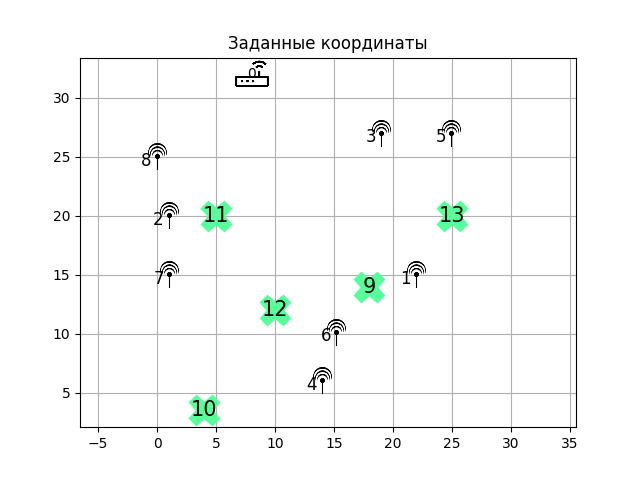
\includegraphics[scale=0.33]{mip_input_data.png}
        \center{\textbf{Множества заданных вершин}}
        
    \end{minipage}  
    \begin{minipage}[c]{0.45\linewidth}
        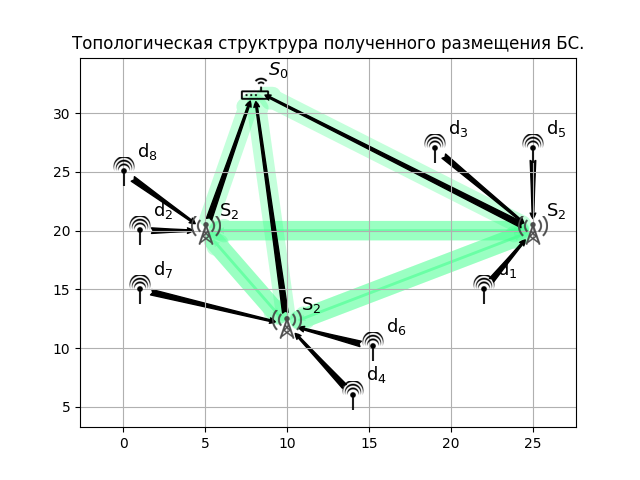
\includegraphics[scale=0.35]{mip_solution.png}
        \center{\textbf{Оптимальное решение}}

    \end{minipage}

    \medskip Математическая модель ЧЦЛП (26) - (31) написана на языке Python и решена в Gurobi Optimization.
    \textit{https://github.com/m0000Amir/BSP-on-plane}
    
\end{frame}

\begin{frame}
    \frametitle{Выводы по Положению 4}
    \fontsize{8pt}{7.2}\selectfont

    В рамках широкого \textbf{класса задач размещения мощностей} во всех представленных задачах размещения присутсвует специфика на связь между всеми узлами. 
    \bigskip

    \textbf{Представлены:}
    \begin{itemize}
        \item математическая модель ЛП для проверки условия допустимого потока информации;
        \item математическая модель ЧЦЛП оптимального размещения базовых станций для контроля множества рассредоточенных объектов.
    \end{itemize}

    \bigskip
    \textbf{Оснонвые публикации:}
    \begin{minipage}[c]{1\linewidth}
        \fontsize{6pt}{7.2}\selectfont
        \begin{enumerate}
            \item \textit{Мухтаров, А. А.Задача размещения базовых станций широкопо­лосной связи для обслуживания заданного множества рассредото­ченных объектов [текст] / А. А. Мухтаров, О. Ю. Першин // Труды 13-го Всероссийского совещания по проблемам управления (ВСПУ XIII, Москва, 2019). — 2019. — с. 2992—2994.};
            
            \item \textit{Мухтаров,А. А.Оптимальное размещение базовых станций широ­кополосной беспроводной сети связи для обслуживания заданного множества рассредоточенных объектов [текст] / А. А. Мухта­ров, О. Ю. Першин // Труды 12-й Международной конференции«Управление развитием крупномасштабных систем» (MLSD’2019,Москва). — 2019. — с. 531—537};
            
        \end{enumerate}
    \end{minipage}

\end{frame}

\begin{frame}
    \frametitle{Выводы}
    
    \begin{enumerate}
        \item разработаны математическая модель ЦЛП и экстремальной комбинаторной модель для оптимального размещения базовых станций при
        проектировании беспроводных широкополосных сетей (БШС) вдоль протяженной транспортной магистрали;
        \item предложен специальный алгоритм МВиГ для решения сформулированной
        экстремальной комбинаторной модели;
        \item разработана итерационная процедура нахождения последовательности лучших
        решений для задачи размещения базовых станций в рамках комплексного
        проектирования БШС вдоль протяженной транспортной магистрали;
        \item разработаны математические модели для задач проектирования БШС с ячеистой
        топологией для обслуживания множества рассредото­ченных объектов;
    \end{enumerate}
\end{frame}

% \section{Публикации}
\begin{frame}
    \frametitle{Публикации}
    \fontsize{7pt}{7.2}\selectfont

    \textbf{Основные результаты} по теме диссертации изложены в \textbf{15} печатных изданиях, \textbf{2} из которых изданы в журналах, рекомендованных \textbf{ВАК}, \textbf{3} — в периодических научных журналах, индексируемых \textbf{Web of Science и Scopus}, \textbf{10} — в сборниках трудов конференции, индексируемых \textbf{РИНЦ}. Зарегистрирована \textbf{1} программа для \textbf{ЭВМ}. 
    
    \bigskip
    
    В изданиях из списка \textbf{ВАК}: 
    \begin{enumerate}
        \item \textit{Иванов,Р. Е.Задача оптимального размещения заданного множе­ства базовых станций беспроводной сети связи с линейной топо­логией [текст] / Р. Е. Иванов, А. А. Мухтаров, О. Першин //Автоматизация, телемеханизация и связь в нефтяной промышлен­ности. — 2019. — т. 549, No 4. — с. 39—45.}
        \item \textit{Оптимальное размещения базовых станций в рамках комплексного проектирования беспроводной сети [Текст] / О. Ю. Першин, В. М. Вишневский, А. А. Мухтаров, А. А. Ларионов // Информационные технологии и вычислительные системы. — 2022. — No 1. — С. 12—25.}
    \end{enumerate}

    \bigskip

    В изданиях, входящих в международную базу цитирования \textbf{WoS и Scopus}:

    \begin{enumerate}
        \item \textit{Ivanov,R.A Problem of Optimal Location of Given Set of Base Sta­tions in Wireless Networks with Linear Topology[текст]/ R. Ivanov,A. Mukhtarov, O. Pershin // Communications in Computer and Infor­mation Science. –– 2019. –– Vol. 1141 CCIS. –– P. 53––64. –– (Scopus,WoS).}
        \item  \textit{On Optimal Placement of Base Stations in Wireless Broadband Net­works to Control a Linear Section with End-to-End Delay Limited[текст]/ A. Mukhtarov [et al.] // Communications in Computer andInformation Science. –– 2020. –– Vol. 1337. –– P. 30––42.}
        \item \textit{Larionov, A. A. The calibration method of a tandem queueing model with PH service time using NS-3 simulation of a multihop wireless network [Текст] / A. A. Larionov, A. A. Mukhtarov, A. M. Sokolov // Journal of Physics: Conference Series. –– 2021. –– Vol. 2091, no. 1. –– P. 012030.}
    \end{enumerate}
    
\end{frame}

\begin{frame}
    \frametitle{Апробация работы}
    \begin{enumerate} % https://tex.stackexchange.com/a/476052/104425
        \fontsize{8pt}{7.2}\selectfont
        \item «Губкинский университет в решении вопросов нефтегазовой отрасли России» (Москва, 17-21 сентября 2018); 
        \item «13-е Всероссийское совещание по проблемам управления» (Москва, 17-20 июня 2019); 
        \item «International Conference on Distributed Computer and Communication Networks: Control, Computation, Communications» (Москва, 22-27 сентября 2019), 
        \item «Губкинский университет в решении вопросов нефтегазовой отрасли России» (Москва, 24-26 сентября 2019); 
        \item «Conference Management of Large-Scale System Development» (Москва, 1-3 октября 2019); 
        \item «Information and Telecommunication Technologies and Mathematical Modeling of High-Tech Systems» (Москва, 13-17 апреля 2020); 
        \item «Computer-aided technologies in applied mathematics» (Томск, сентябрь 2020);
        \item «International Conference on Distributed Computer and Communication Networks: Control, Computation, Communications» (Москва, 14-18 сентября 2020); 
        \item «Information and Telecommunication Technologies and Mathematical Modeling of High-Tech Systems» (Москва, 19-23 апреля 2021);
        \item «5th International Scientific Conference on Information, Control, and Communication Technologies» (Астрахань, 4-7 октября 2021)
      \end{enumerate}
\end{frame}

\begin{frame}[plain, noframenumbering]
    \frametitle{Положения}
    \begin{enumerate} % https://tex.stackexchange.com/a/476052/104425
        \item Формулировка задачи оптимального размещения базовых станций при проектировании беспроводных широкополосных сетей (БШС) вдоль протяженных транспортных магистралей в виде целочисленного линейного программирования (ЦЛП) и в виде комбинаторной модели в экстремальной форме.
   
        \item Специальный алгоритм типа ветвей и границ для решения сформулированной экстремальной комбинаторной задачи.
        \item Итерационная процедура нахождения последовательности лучших решений для задачи размещения базовых станций в рамках комплексного проектирования БШС вдоль протяженных транспортных магистралей.
        \item Математические модели для задач проектирования БШС с ячеистой топологией для обслуживания множества рассредоточенных объектов.
      \end{enumerate}
\end{frame}


\begin{frame}[plain, noframenumbering]
    \frametitle{Замечания и вопросы к диссертационной работе}
    \fontsize{8pt}{7.2}\selectfont
    \textbf{д.т.н., профессор Степанов Сергей Николаевич}

    \bigskip

    \begin{enumerate}
        \item Для оценки межконцевых задержек с помощью аналитической модели, предполагается, что на каждую базовую станцию пакеты поступают с одинаковой интенсивностью. В реальных сетях нагрузка на каждый узел может отличаться.
        \item В предложенном алгоритме типа ветвей и границ рассматривается размещения множества базовых станций. В качестве развития тематики исследования, в дальнейшем было бы интересно выбирать базовые станции из заданного множества типов базовых станций в ходе поиска оптимального размещения.
        \item Было бы интересно рассмотреть влияние особенностей рельефа на размещение базовых станций. Автор исходит из упрощенного предположения (впрочем, вполне справедливого для модельной задачи) о постоянстве дальности связи между станциями, хотя в реальности стоит учитывать наличие прямой видимости, преград и пр.
        
    \end{enumerate}
\end{frame}


\begin{frame}[plain, noframenumbering]
    \frametitle{Замечания и вопросы к диссертационной работе}
    \fontsize{8pt}{7.2}\selectfont
    \textbf{д.т.н., профессор Пащенко Фёдор Фёдорович}

    \bigskip

    \begin{enumerate}
        \item В 1.4.4 не хватает подробного описания используемых методов машинного обучения.
        \item В работе не представлены другие характеристики производительности сети в качестве ограничений задачи, помимо оценки межконцевой задержки.
        \item В представленном в главе 1 расчете межконцевой задержки в сети предполагается, что на каждую фазу поступает одинаковый трафик с интенсивностью лямбда. Такое ограничение, безусловно, удобно для расчетов. Однако, необходимо рассмотреть влияния на задержку поступление разного трафика на разные станции. Например, большого трафика на конечные и отдельные промежуточные узлы, и малого трафика на остальные.
        \item В работе присутствуют ряд орфографических и грамматических ошибок.
        
    \end{enumerate}
\end{frame}



\begin{frame}[plain, noframenumbering]
    \frametitle{Замечания и вопросы к диссертационной работе}
    \fontsize{8pt}{7.2}\selectfont
    \textbf{д.т.н., академик РАН Кузнецов Николай Александрович}

    \bigskip

    \begin{enumerate}
        \item Точность аналитической модели в диссертации проверялась сравнением с имитационной моделью беспроводной сети в среде NS-3. Насколько подробно в имитационной модели учитывалась протоколы беспроводной сети?
        \item При использовании модели распространения сигналов для оценки дальности телекоммуникационной связи учитывался ли эффект Доплера?
        \item На страницах 95 и 96 в описание входной конфигурации задачи удобно было бы предоставить в виде листинга кода, а не в виде картинки.
        %  
        
    \end{enumerate}
\end{frame}


\begin{frame}[plain, noframenumbering]
    \frametitle{Замечания и вопросы к диссертационной работе}
    \fontsize{8pt}{7.2}\selectfont
    \textbf{д.т.н., профессор Абросимов Леонид Иванович}

    \bigskip

    \begin{enumerate}
        \item В главе 2 не хватает примеров. Для чтения работы было бы лучше, если в главе использовался один численный пример и для задачи ЦЛП, и для метода ветвей и границ, подобно тому, как это сделано в главе 3. Хотя автор привел подробное описание применения предложенных методов к решению практической задачи с данными реального оборудования в главе 4, более простой пример в главе 2 сделал бы работу более читаемой и наглядной.
        \item Также усилить модель можно было, если бы в задаче также учитывалась интерференция в том случае, если станции работают в полудуплексном режиме. В сетях IEEE 802.11 использование одного канала разными станциями может очень существенно влиять на пропускную способность.
        \item Для оценки предложенного алгоритма используется только мера количества пройденных узлов в ходе поиска. В работе отсутствуют другие варианты оценок алгоритма.
        \item На странице 95 и странице 101 присутствуют орфографические ошибки.
        
    \end{enumerate}
\end{frame}


\begin{frame}[plain, noframenumbering]
    \frametitle{Замечания и вопросы к диссертационной работе}
    \fontsize{8pt}{7.2}\selectfont
    \textbf{д.т.н., профессор Самуйлов Константин Евгеньевич}

    \bigskip

    \begin{enumerate}
        \item В 1.4.1 поверхностно описан алгоритм DCF протокола 802.11, требуется более конкретное описание функции. Нечетко описан алгоритм backoff.
        \item Реализация имитационных моделей, упомянутых в главе 1, изложено в объеме, затрудняющем целостное восприятие текста.
        \item Автор утверждает, что модели СМО с конечным размером буфера (M/M/1/N, M/PH/1/N) сложно исследовать аналитически, что не подтверждено какими-либо ссылками на литературные источники. 
        
        \item В качестве входных параметров задачи поиска оптимального размещения используются множество заранее отобранных возможных точек размещения базовых станций. Неясно по каким важным критериям отбираются данные координаты размещения базовых станций.
        
    \end{enumerate}
\end{frame}


\begin{frame}[plain, noframenumbering]
    \frametitle{Замечания и вопросы к диссертационной работе}
    \fontsize{8pt}{7.2}\selectfont
    \textbf{д.т.н., старший научный сотрудник Фархадов Маис Паша Оглы}

    \bigskip

    \begin{enumerate}
        \item Необходимо пояснить, почему модель M/PH/1/N дает наибольшее отклонение от результатов имитационной модели, по сравнению с моделями M/M/1/N (которая является частным случаем M/PH/1/N) и M/M/1.
        \item В главе 4 все примеры расчета дальности телекоммуникационной связи представлены с использованием только теоретической модели распространения сигнала в свободном пространстве. Отсутствуют примеры использования других моделей распространения из главы 1.
        \item В диссертации имеются стилистические неточности.
        
    \end{enumerate}
\end{frame}


\begin{frame}[plain, noframenumbering]
    \frametitle{Отзыв ведущей организации}
    \fontsize{8pt}{7.2}\selectfont
    \textbf{Санкт-Петербургский государственный университет телекоммуникаций им. проф. М. А. Бонч-Бруевича}

    \bigskip

    \begin{enumerate}
        \item Материал в автореферате освещен не совсем равномерно, третья и четвертая глава описаны менее полно по сравнению с главой 2.
        \item Для разработанного алгоритма не совсем ясно, возможно ли проводить оценку других характеристик производительности сети, например, пропускную способность, в ходе поиска оптимального размещения базовых станций.
        \item В главе 4 отсутствуют численные примеры задач размещения базовых станций для сотовых сетей.
        \item Присутствует незначительное число орфографических ошибок и опечаток.
        
    \end{enumerate}
\end{frame}


\begin{frame}[plain, noframenumbering]
    \frametitle{Внешние отзывы}
    \fontsize{8pt}{7.2}\selectfont
    \textbf{д.т.н., профессор РАН Мещеряков Роман Валерьевич}

    \bigskip

    \begin{enumerate}
        \item Для расчета дальности телекоммуникационной связи описан целый ряд моделей распространения радиосигналов. Неясно почему в расчетах используется только модель распространения радиосигналов в свободном пространстве.
        \item Оценка межконцевых задержек проводится с использованием многофазной сети с экспоненциальными распределениями и конечным буфером. Необходимо рассмотреть более сложные модели многофазных сетей массового обслуживания для использования в разработанном алгоритме.
        \item Оценка адекватности применения сетей массового обслуживания для моделирования беспроводной сети проводилась автором c использованием имитационной модели в среде NS-3. Результаты аналитического и имитационного моделирования не проверялись в рамках эксперимента на реальных сетях.
        \item В качестве оценки эффективности разработанного алгоритма типа ветвей и границ используется мера количества пройденных узлов в ходе поиска оптимального решения. Необходимо проверить разработанный алгоритм по критерию времени счета. Необходимо проверить быстродействие разработанного алгоритма.
        \item В диссертационной работе присутствует ряд орфографических ошибок.
        
    \end{enumerate}
\end{frame}

\begin{frame}[plain, noframenumbering]
    \frametitle{Внешние отзывы}
    \fontsize{8pt}{7.2}\selectfont
    \textbf{д.т.н., профессор Ермолаев Александр Иосифович}

    \bigskip

    \begin{enumerate}
        \item Желательно было бы привести примеры практических задач проектирования «сотовых» сетей. Например, проектирование БШС для наблюдения за технологическими объектами на нефтяных и газовых промыслах.
        \item Результаты численных экспериментов приведены не для всех, рассмотренных в диссертации задач.
        \item В работе предлагается полезная для практики процедура построения последовательности лучших решений на основе алгоритма МВиГ решения задачи размещения базовых станций на линейном отрезке, представленной в комбинаторной форме. Но в диссертации не указано, что такая же процедура может быть построена для моделей ЦЛП, например, на основе метода Ленд и Дойг.
        
        
    \end{enumerate}
\end{frame}